\chapter{Αντιστοίχιση με Αλγορίθμους Θεωρίας Παιγνίων - Ομοσπονδιακή Μάθηση}

Στόχος της παρούσας διπλωματικής εργασίας είναι να δημιουργήσουμε από το οικοσύστημα μας (εξυπηρετητές, κρίσιμα σημεία, κόμβους, που θα περιγραφούν και στη συνέχεια), ένα συνασπισμό για κάθε εξυπηρετητή. Σε κάθε τέτοιο συνασπισμό επιχειρούμε να πετύχουμε την καλύτερη δυνατή επίδοση για το μοντέλο αναγνώρισης και ταξινόμησης εικόνας του εξυπηρετητή, μέσω Ομοσπονδιακής Μάθησης, εκπαιδεύοντας έτσι στο δίκτυό μας πολλαπλά μοντέλα. Ως πρώτο κομμάτι, θα αναφερθούμε στην χρήση Θεωρίας Παιγνίων για την αντιστοίχιση κόμβων - εξυπηρετητών, με στόχο την βελτιστοποίηση των αποτελεσμάτων της Ομοσπονδιακής Μάθησης. Συνεπώς, όπως θα περιγράψουμε και στη συνέχεια, η εκτέλεση της προσομοίωσης θα ακολουθήσει δύο φάσεις: η πρώτη αφορά την αντιστοίχιση των κόμβων με τους εξυπηρετητές, και αφού αυτή ολοκληρωθεί περνάμε στην δεύτερη φάση, αυτή της Ομοσπονδιακής Μάθησης, όπου κάθε εξυπηρετητής θα επιχειρήσει να εκπαιδεύσει το μοντέλο του με την βοήθεια των κόμβων που του ανατέθηκαν.

\section{Προσομοίωση}

Η προσομοίωση αφορά κομμάτι ενός ευρύτερου δικτύου που προσπαθεί να εξασφαλίσει την δημόσια ασφάλεια σε περιπτώσεις φυσικών καταστροφών. Οι εξυπηρετητές, θέλοντας να μάθουν να αναγνωρίζουν έγκαιρα κινδύνους για τους πολίτες, προσπαθούν να εκμαιεύσουν πληροφορία από κόμβους που έχουν βρεθεί κοντά σε τέτοιες καταστροφές. Ο όρος "κόμβος" είναι ένας ευρύτερος όρος που αναθέτουμε είτε σε κινητά τηλέφωνα πολιτών, είτε κάμερες ασφαλείας καταστημάτων, είτε στιγμιότυπα από ειδησεογραφική κάλυψη κ.α., που διαθέτουν φωτογραφίες από την εκάστοτε φυσική καταστροφή. Στην δική μας περίπτωση, μας αφορούν φυσικές καταστροφές φωτιών, πλημμύρων και σεισμών. Συνεπώς στόχος του δικτύου μας είναι για παράδειγμα, να εντοπίζει έγκαιρα κάποια φωτιά ή πλυμμύρα και να ειδοποιεί τις πυροσβεστικές δυνάμεις, αλλά και τους κοντινούς σε αυτή πολίτες για να τους προειδοποιήσει και να τους καθοδηγήσει σε ασφαλή περιοχή. Αντίστοιχα σε περιπτώσεις σεισμών, να εντοπίζει κτίρια που έχουν υποστεί σοβαρές ζημιές και να ειδοποιεί για την άμεση εκκένωσή τους και την απομάκρυνση των πολιτών από αυτά. 

Η προσομοίωσή μας ακολουθεί το εξής σενάριο. Έχουμε 3 εξυπηρετητές όπου ο καθένας επιθυμεί να εκπαιδεύσει ένα μοντέλο αναγνώρισης - ταξινόμησης εικόνας. Ο πρώτος προσπαθεί να αναγνωρίσει εικόνες φωτιάς, ο δεύτερος πλημμύρων και ο τρίτος σεισμών. Στο οικοσύστημά μας έχουμε και Κ κρίσιμα σημεία, τα οποία το καθένα αφορά μια από τις προαναφερθείσες φυσικές καταστροφές. Στο πλαίσιο της εργασίας αυτής χρησιμοποιήθηκε $K=3$, δηλαδή ένα σημείο για κάθε φυσική καταστροφή. Επιπλέον, γύρω από αυτά τα σημεία, έχουμε Ν κόμβους, οι οποίοι διαθέτουν φωτογραφίες από φυσικές καταστροφές, αλλά και από την καθημερινή τους χρήση, τις οποίες θα χρησιμοποιήσουν για να συμμετέχουν στην Ομοσπονδιακή Μάθηση που θα ακολουθήσει.

\subsection{Περιγραφή}

Στο πλαίσιο που περιγράψαμε παραπάνω θα διακρίνουμε 3 ξεχωριστές περιπτώσεις, όσον αφορά την περιοχή στην οποία τοποθετείται το δίκτυό μας. Έτσι διακρίνουμε σε Αστικές Περιοχές, Μικροαστικές Περιοχές και Αγροτικές Περιοχές και στη συνέχεια θα περιγράψουμε και αναλυτικά την διαφορά τους στην υλοποίηση. 

\begin{figure}[ht]
    \centering
    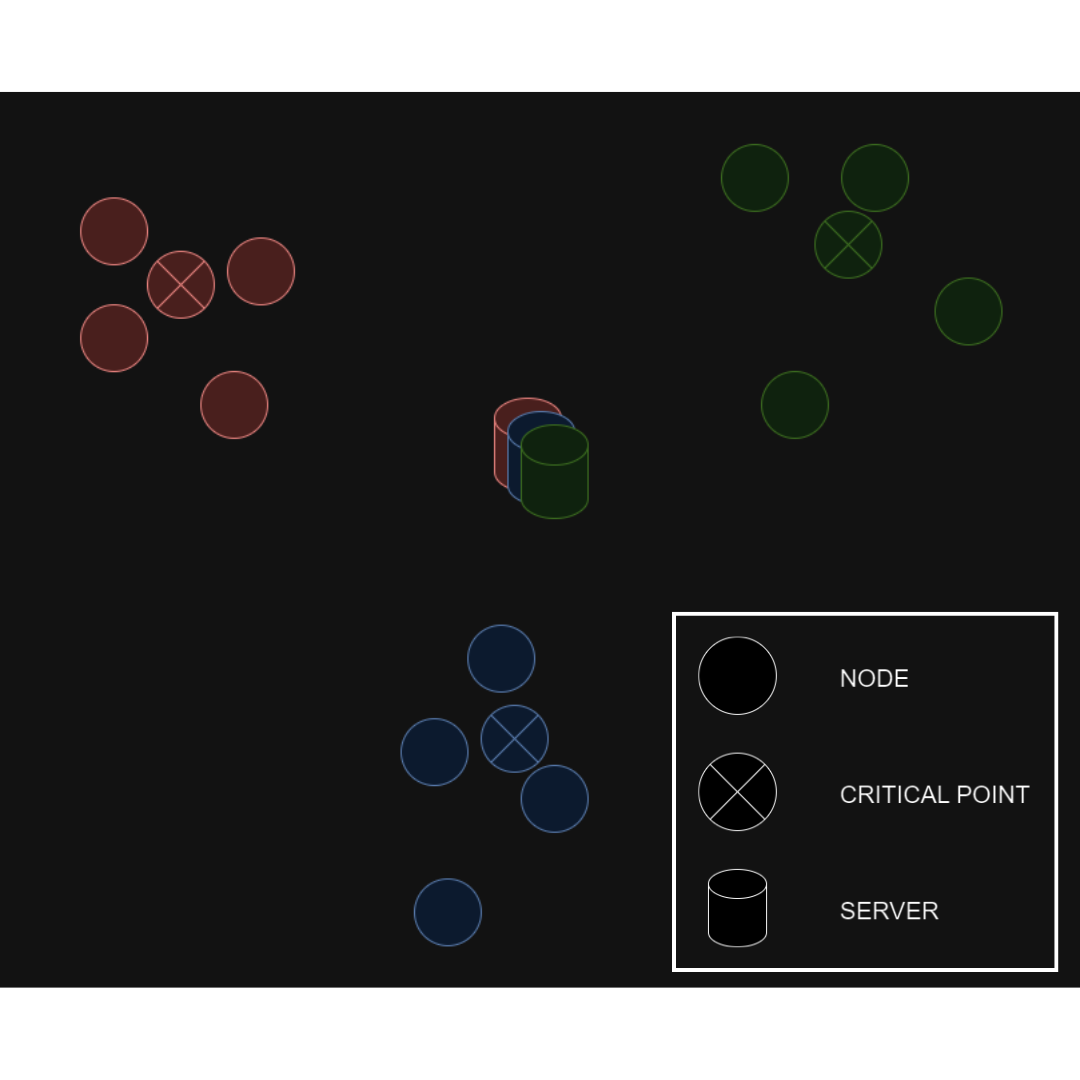
\includegraphics[width=\textwidth]{figures/chapter2/topology+ypomn.png}
    \vspace{-1cm}
    \caption{Παράδειγμα Τοπολογίας Κόμβων και Εξυπηρετητών (Κόκκινο - Φωτιά, Μπλέ - Πλημμύρα, Πράσινο - Σεισμός)}
    \label{fig46}
\end{figure}

 Ξεκινώντας από την τοπολογία του συστήματός μας, τοποθετούμε αρχικά τους εξυπηρετητές μας στο σημείο (0,0,0), στο κέντρο του οικοσυστήματός μας. Κάθε εξυπηρετητής διαθέτει $\ceil*{\frac{N}{3}}$ χρηματικά αποθέματα, με τα οποία μπορεί να προσελκύσει σε αυτόν κόμβους. Επιπλέον, θέτουμε ένα ανώτατο όριο κόμβων για κάθε εξυπηρετητή. Έτσι, κάθε εξυπηρετητής μπορεί να χτίσει ένα συνασπισμό το πολύ $\ceil*{\frac{N}{3}}$ κόμβων. Μπορεί, λοιπόν, να χρηματοδοτήσει το πολύ το $\frac{1}{3}$ των κόμβων, χαρακτηριστικό που μας βοηθά στην διατήρηση της ισορροπίας μεταξύ των εξυπηρετητών. Έπειτα, σε έναν κύβο ακμής μήκους 2, γύρω από το (0,0,0) επιλέγουμε 3 σημεία, ένα για κάθε φυσική καταστροφή. Σε αυτά θεωρούμε πως έχει συμβεί η εκάστοτε φυσική καταστροφή και άρα κόμβοι γύρω από αυτά θα έχουν χρήσιμη πληροφορία για τους εξυπηρετητές μας. Εξασφαλίζουμε επίσης πως τα σημεία δεν είναι πολύ κοντά στους εξυπηρετητές. Σε μια τέτοια περίπτωση, όπως θα δούμε και στην διαδικασία της αντιστοίχισης, οι κόμβοι γύρω από αυτό θα παρουσίαζαν πολύ μεγαλύτερη χρησιμότητα στο σύστημα, απλώς επειδή βρίσκονται κοντά στους εξυπηρετητές και είναι "φθηνή" η επικοινωνία με αυτούς. Έτσι, για να διασφαλίσουμε μια ισορροπία ορίζουμε ως ελάχιστη απόσταση από τους εξυπηρετητές $d_{min} = 0.3$. Επιπλέον, για ρεαλιστικούς κυρίως λόγους, ορίζουμε ως ελάχιστη απόσταση μεταξύ δύο κρίσιμων σημείων ίση με $d_{min} = 0.8$. 

Στη συνέχεια, μας απομένει να τοποθετήσουμε τους κόμβους μας γύρω από τα κρίσιμα σημεία. Η λογική που ακολουθούμε εδώ είναι η εξής: ανάλογα με την περιοχή που βρισκόμαστε (Αστική, Προαστιακή, Αγροτική) οι κόμβοι είναι λιγότερο ή περισσότερο αραιοί γύρω από το κάθε κρίσιμο σημείο. Συνεπώς, θέτουμε 3 όρια: $rural\_limit = 12, suburban\_limit = 21$ και $urban\_limit = 30$. Έτσι, για τις αγροτικές περιοχές όταν έχουμε πάνω από 12 κόμβους, αρχίζουμε να τοποθετούμε τους υπόλοιπους κόμβους πιο αραιά. Αντίστοιχα, το όριο για τις μικροαστικές περιοχές είναι 21 και για τις αστικές 30. Στις προσομοιώσεις μας, το μεγαλύτερο Ν που θα χρησιμοποιήσουμε είναι το $N = 30$. Επιπλέον, για δική μας διευκόλυνση ο κόμβος με διακριτικό id ανατίθεται γύρω από το κρίσιμο σημείο $id\mod3$, και όσο μεγαλύτερο το id τόσο πιο μακριά είναι από το κρίσιμο σημείο. Άρα οι τρεις πρώτοι κόμβους είναι πολύ κοντά στα κρίσιμα σημεία τους, οι τρεις επόμενοι λίγο πιο μακριά κ.ο.κ. Όπως αναφέραμε, όταν για κάθε μία από τις διαφορετικές περιοχές ξεπεράσουμε το αντίστοιχο όριο, αρχίζουμε να προσθέτουμε πιο αραιούς-μακρινούς κόμβους. Με τον τρόπο αυτό μοντελοποιούμε το γεγονός πως σε περιοχές που βρίσκονται σε προάστια ή στην εξοχή, οι γειτονικοί στο κρίσιμο σημείο κόμβοι είναι λιγότεροι, αλλά είναι πιθανό να υπάρχουν και άλλοι, όμως πιο απομακρυσμένοι, κόμβοι. Σε κάθε περίπτωση, ολοκληρώνοντας την τοπολογία μας καταλήγουμε σε 3 κρίσιμα σημεία γύρω από τους εξυπηρετητές μας, όπου το κάθε ένα έχει γύρω του κόμβους. Ανάλογα την περιοχή όπου διατίθεται το δίκτυό μας, οι κόμβοι αυτοί είναι λιγότερο ή περισσότερο αραιοί. Είναι σημαντικό να επισημάνουμε προφανώς, πως όσο πιο κοντά είναι ένας κόμβος σε ένα κρίσιμο σημείο, τόσο πιο αξιόπιστος είναι για την πληροφορία που διαθέτει για αυτό, σημαντικό χαρακτηριστικό όπως θα δούμε και στη συνέχεια για την αντιστοίχιση κόμβων-εξυπηρετητών. Τέλος, σημειώνουμε πως ο κάθε κόμβος διαθέτει δύο παραμέτρους $a_n$ και $q_n$, οι οποίες εκφράζουν τον συντελεστή αποτελεσματικής χωρητικότητας του επεξεργαστή του κόμβου και τον αριθμό κύκλων Κεντρικής Μονάδας Επεξεργασίας (ΚΜΕ) που απαιτούνται για την εκτέλεση ενός δείγματος δεδομένων αντίστοιχα.

\newpage

Παρακάτω παρουσιάζονται παραδείγματα των διαφορετικών τοπολογιών - σεναρίων: 

\begin{figure}[H]
    \centering
    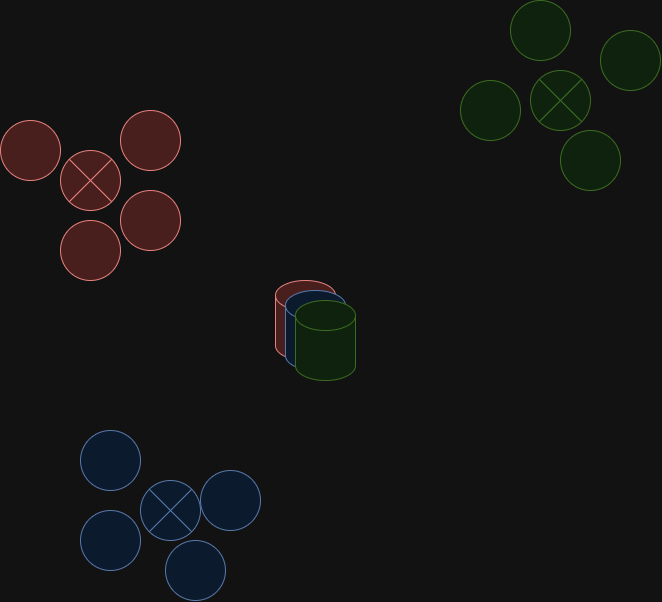
\includegraphics[width=0.7\textwidth]{figures/chapter2/urban.drawio.png}
    \caption{Αστική Περιοχή με 12 κόμβους}
    \label{fig47}
\end{figure}

\begin{figure}[H]
    \centering
    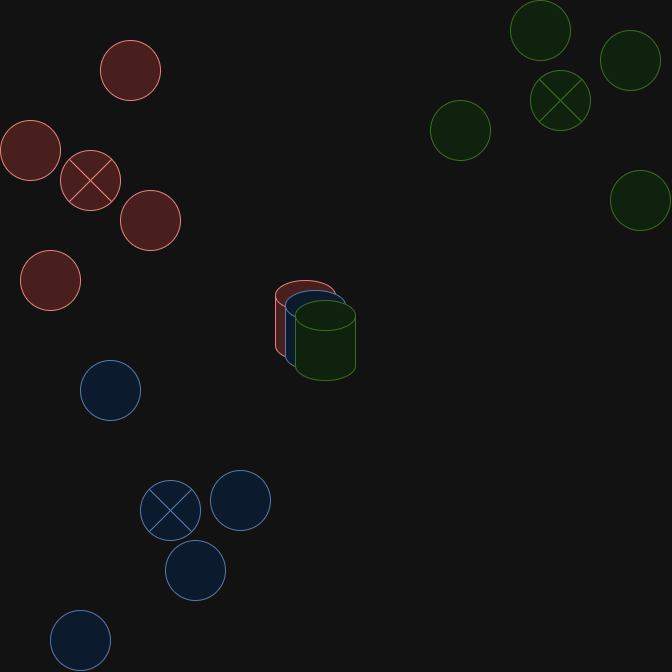
\includegraphics[width=0.7\textwidth]{figures/chapter2/suburban.drawio.png}
    \caption{Προαστιακή Περιοχή με 12 κόμβους}
    \label{fig48}
\end{figure}

\newpage

\begin{figure}[H]
    \centering
    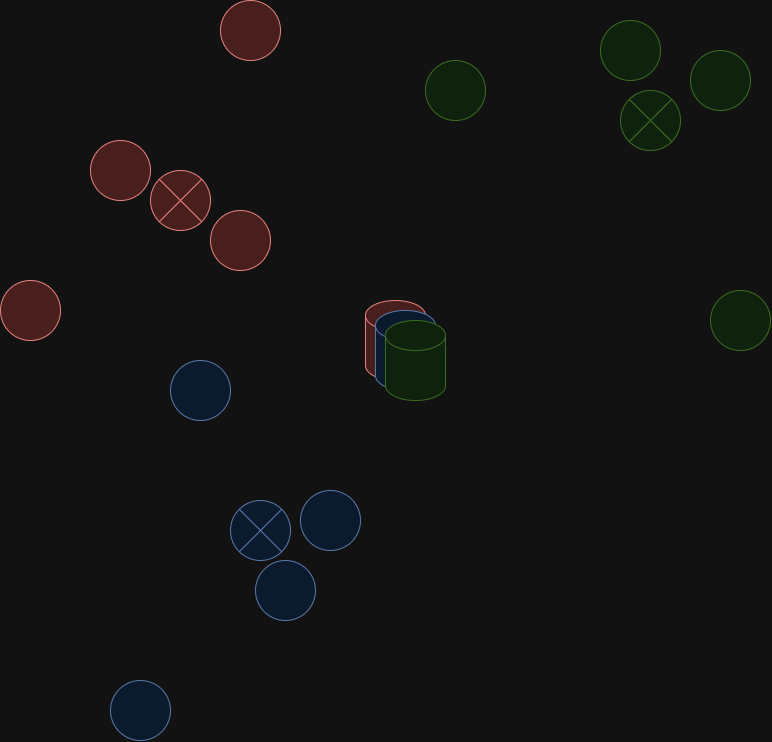
\includegraphics[width=0.7\textwidth]{figures/chapter2/rural.drawio.png}
    \caption{Αγροτική Περιοχή με 12 κόμβους}
    \label{fig49}
\end{figure}

\subsection{Υλοποίηση}

Για να συγκρίνουμε την επίδοση του αλγορίθμου μας σε διαφορετικές περιοχές (αστικό, προαστιακό ή υπαίθριο περιβάλλον) θα πρέπει να εξασφαλίσουμε μια δίκαιη και ορθή σύγκριση. Όπως αναφέραμε παραπάνω, έχουμε δύο είδη κόμβων για κάθε περιοχή, γειτονικοί - "καλοί" και απομακρυσμένοι - "κακοί". Στην αστική περιοχή και οι 30 κόμβοι, που μπορούν να μπουν ως μέγιστο όριο, θεωρούνται "καλοί" και άρα είναι σχετικά κοντά στο κρίσιμο σημείο τους. Αντίστοιχα, στην προαστιακή περιοχή μέχρι και τον 21ο κόμβο, οι κόμβοι θεωρούνται "καλοί", ενώ, σε περίπτωση που το Ν ξεπεράσει το 21, αρχίζουν να εισέρχονται στο σύστημά μας "κακοί" κόμβοι, οι οποίοι τοποθετούνται τουλάχιστον 0.2 μακριά από το κρίσιμο σημείο τους. Τέλος, στην αγροτική περιοχή, μέχρι και τον 12ο κόμβο, οι κόμβοι θεωρούνται "καλοί", ενώ, σε περίπτωση που το Ν ξεπεράσει το 12, αρχίζουν να εισέρχονται στο σύστημά μας "κακοί" κόμβοι, οι οποίοι τοποθετούνται τουλάχιστον 0.3 μακριά από το κρίσιμο σημείο τους. Συνεπώς, έστω πως έχουμε τον κόμβο i, τον οποίο θα πρέπει να δημιουργήσουμε. Αν το i είναι μικρότερο ή ίσο του 12 θα πρέπει όλες οι περιοχές να έχουν ίδιο κόμβο i και να μην ξαναδημιουργηθούν τυχαίοι κόμβοι i σε κάθε περιοχή. Με την ίδια λογική όταν το i είναι μικρότερο ή ίσο του 21 (αλλά μεγαλύτερο του 12), θα πρέπει οι κόμβοι i να είναι ίδιοι για την αστική και προαστική περιοχή, αλλά για την αγροτική περιοχή θα πρέπει να δημιουργηθεί ένας "κακός" κόμβος i. Τέλος, για διευκόλυνση μας, υπολογίζουμε και αποθηκεύουμε τις αποστάσεις κάθε κόμβου από τους εξυπηρετητές μας και την σημασία κάθε κόμβου για τον κάθε εξυπηρετητή. Τέλος, όσον αφορά τις παραμέτρους $a_n$ και $q_n$ θέτουμε:

\begin{itemize}
    \item $a_n = 2 \times 10^{(-28)} \times \text{random.uniform(0.95, 1.05)}$
    \item $q_n = 20 \times \text{random.uniform(0.95,1.05)}$
\end{itemize}

\noindent όπως αναφέρεται και σε αντίστοιχη προσομοίωση (\lcite{charatsaris2023accuracy}).

\section{Αντιστοίχιση με Θεωρία Παιγνίων}

Ως πρώτος μηχανισμός για την αντιστοίχιση κόμβων-εξυπηρετητών χρησιμοποιήθηκε η Θεωρία Παιγνίων. Στόχος ήταν να κατασκευαστεί ένα περιβάλλον με κανόνες, μέσα στο οποίο οι παίκτες-κόμβοι θα ανταγωνίζονται και θα ενεργούν για να επιτύχουν την καλύτερη δυνατή αμοιβή για εκείνους. Αντίστοιχα, οι εξυπηρετητές διαθέτοντας τους χρηματικούς πόρους τους στους κόμβους, προσπαθούν και αυτοί με τη σειρά τους να βελτιστοποιήσουν την δική τους απολαβή. Πιο αναλυτικά την διαδικασία θα περιγράψουμε παρακάτω.

\subsection{Συνάρτηση Χρησιμότητας}

Αρχικά θα πρέπει να εξηγήσουμε τον τρόπο με τον οποίο κάθε κόμβος, αλλά και εξυπηρετητής αντιλαμβάνεται το συμφέρον του στο δίκτυό μας. Έτσι χτίζουμε μία Συνάρτηση Χρησιμότητας. Κάθε κόμβος $n$ έχει μια ποσότητα συλλεγμένων δεδομένων $D_n$ [bits], και η σημασία των δεδομένων τους ορίζεται ως:

\vspace{-5pt}

\begin{equation}
c_{n,k}=\frac{\min\limits_{\forall n} ||L_n-L_k||}{||L_n-L_k||}
\label{eq1}
\end{equation}

\noindent
όπου $L_n = (x_n,y_n,z_n)$ [απόσταση σε m] και $L_k = (x_k,y_k,z_k)$ [απόσταση σε m], με $k$ το εκάστοτε κρίσιμο σημείο, αποτυπώνοντας πόσο κοντά στα κρίσιμα σημεία έχουν συλλεχθεί τα δεδομένα. Για κάθε έναν από τους τρεις εξυπηρετητές $s$ υπολογίζουμε την σημασία των δεδομένων του κάθε κόμβου ως:

\begin{equation}
c_{n,s}=\max\limits_{\forall k \in s} c_{n,k}
\label{eq2}
\end{equation}

\noindent
Όπως αναφέραμε, στην Ομοσπονδιακή Μάθηση, κάθε κόμβος $n$ εκπαιδεύει ένα τοπικό μοντέλο βασισμένο στον εξυπηρετητή $s$ που έχει επιλεγεί και αναφέρει το αποτέλεσμα της εκπαίδευσης σε αυτόν. Ο ρυθμός δεδομένων κάθε κόμβου $n$ όταν εκφορτώνει το τοπικό μοντέλο στον εξυπηρετητή $s$ δίνεται ως εξής:

\vspace{-5pt}

\begin{equation}
R_{n,s} = B \log_2(1 + \frac{g_{n,s} P_{n,s}}{\sum \limits_{n'\in s} g_{n',s}P_{n',s} + I_0}) \quad [bps]
\label{eq3}
\end{equation}

\vspace{-3pt}

\noindent
όπου $g_{n,s}$ δηλώνει το κέρδος καναλιού στη ζεύξη επικοινωνίας μεταξύ $n$ και $s$, $P_{n,s}$ [W] είναι η ισχύς εκπομπής του κόμβου, $B$ [Hz] είναι το εύρος ζώνης επικοινωνίας, και $I_0$ είναι ο λευκός προσθετικός θόρυβος (AWGN) μηδενικής μέσης τιμής. \lcite{charatsaris2023accuracy}

Η κατανάλωση ενέργειας ενός κόμβου $n$ για να εκπαιδεύσει τοπικά το επιλεγμένο παγκόσμιο μοντέλο υπολογίζεται ως εξής:

\vspace{-5pt}

\begin{equation}
E_n=\frac{a_n}{2}q_nD_nf_n^2 [J]
\label{eq4}
\end{equation}

\vspace{-3pt}

\noindent
όπου $a_n$ είναι ο συντελεστής χωρητικότητας του επεξεργαστή του κόμβου $n$, $q_n$ είναι οι κύκλοι της Κεντρικής Μονάδα Επεξεργασίας (ΚΜΕ) που απαιτούνται για την εκτέλεση ενός δείγματος δεδομένων, και $f_n$ [κύκλοι ΚΜΕ/δευτερόλεπτο] είναι η συχνότητα της ΚΜΕ της συσκευής του κόμβου $n$. \lcite{charatsaris2023accuracy} 

Η κατανάλωση ενέργειας λόγω της μετάδοσης της ενημέρωσης του τοπικού μοντέλου υπολογίζεται ως εξής:

\vspace{-5pt}

\begin{equation}
E_{n,s}=\frac{Z(\mathbf{w}n)P{n,s}}{R_{n,s}}[J]
\label{eq5}
\end{equation}

\vspace{-3pt}

\noindent
όπου $Z(\mathbf{w}_n)$ [bits] είναι τα δεδομένα των παραμέτρων του τοπικού μοντέλου $\mathbf{w}_n$ που μεταδίδονται για την ενημέρωση του κεντρικού μοντέλου του εξυπηρετητή $s$. \lcite{charatsaris2023accuracy}

Τέλος, ο κάθε κόμβος απολαμβάνει μια χρηματική απολαβή με βάση την σημασία των δεδομένων του, αλλά και με βάση τους υπόλοιπους κόμβους που ανήκουν στην ομοσπονδία του εξυπηρετητή:

\vspace{-5pt}

\begin{equation}
Pnt_{n,s}=\frac{c_{n,s}P_s}{\sum \limits_{n'\in s} c_{n',s}}
\label{eq6}
\end{equation}

\vspace{-3pt}

Κάθε κόμβος βιώνει μια χρησιμότητα από τη συμμετοχή του στη διαδικασία αντιστοίχισης κόμβων-εξυπηρετητών που εξαρτάται από: (i) τα χαρακτηριστικά επικοινωνίας, δηλαδή τον επιτευχθέντα ρυθμό δεδομένων για την αναφορά του ενημερωμένου τοπικού μοντέλου $\mathbf{w}n^i$ στον εξυπηρετητή ($\hat{R}{n,s}$), (ii) το χρηματικό εισόδημα που λαμβάνεται από τον εξυπηρετητή για την παροχή κινήτρων στον κόμβο για την εκπαίδευση του τοπικού μοντέλου ($\hat{Pnt}_{n,s}$) και το σταθερό κίνητρο πρόσληψης που παρέχεται από τον εξυπηρετητή ($\gamma$), (iii) το όφελος της εκμετάλλευσης κρίσιμων δεδομένων για την εκπαίδευση του τοπικού μοντέλου ($\hat{d_n}$), και (iv) το ενεργειακό κόστος για την εκπαίδευση του τοπικού μοντέλου και την αποστολή του στον εξυπηρετητή $(\hat{E}n+\hat{E}{n,s})$. Έτσι, η χρησιμότητα του κόμβου ορίζεται ως εξής:

\vspace{-5pt}

\begin{equation}
    U_{n,s}(D_n)=\alpha \hat{R}_{n,s} + \beta \hat{Pnt}_{n,s} +\gamma + \delta \hat{d_n} -\epsilon (\hat{E}n+\hat{E}{n,s})
    \label{eq7}
\end{equation}

\noindent
όπου ο εξυπηρετητής $s$ προσφέρει $Pnt_{n,s}$ [\$] ως χρηματικό κίνητρο στον κόμβο $n$ για την εκπαίδευση του τοπικού μοντέλου, και $\alpha, \beta, \gamma, \delta, \epsilon \in \mathbb{R}^+$. Για να διασφαλιστεί ότι όλοι οι παράγοντες είναι της ίδιας τάξης μεγέθους, αποτυπώνοντας έτσι δίκαια την επίδρασή τους στη χρησιμότητα του κόμβου, στη χρησιμότητα του κόμβου (Εξίσωση \ref{eq7}) οι $\hat{R}{n,s}, \hat{Pnt}_{n,s}, \hat{E}n$, $\hat{E}{n,s}$ και $\hat{d_n}$ δίνονται από τις εξής κανονικοποιημένες εκφράσεις:

\[\hat{R}{n,s} = \frac{R_{n,s}}{\max \limits_{\forall n, \forall s} { R_{n,s} }}, \hat{Pnt}_{n,s} = \frac{c_{n,s}P_s}{(\sum \limits_{n'\in s} c_{n',s}) \max \limits_{\forall s} P_s}, \hat{d}{n} = \frac{\sum \limits{\forall k \in K} c_{n,k} D_n}{\max \limits_{\forall n} { \sum \limits_{\forall k \in K} c_{n,k} D_n }}\]

\[\hat{E}{n} = \frac{E_{n}}{\max \limits_{\forall n} { E_{n} }},  \hat{E}{n,s} = \frac{E{n,s}}{\max \limits_{\forall n, \forall s} { E_{n,s} }}\]

Από την άλλη πλευρά, κάθε εξυπηρετητής στοχεύει στη μεγιστοποίηση της χρησιμότητας που βιώνουν οι συνδεδεμένοι κόμβοι του, λαμβάνοντας όμως υπόψη το κόστος παροχής κινήτρων πρόσληψης και τον ανταγωνισμό για την πρόσληψη από άλλους εξυπηρετητές εντός του δικτύου πολλαπλών μοντέλων Ομοσπονδιακής Μάθησης. Έτσι, η χρησιμότητα του ομοσπονδιακού εξυπηρετητή είναι:

\vspace{-5pt}

\begin{equation}
U_s(P_s, \mathbf{P_{-s}}) = \frac{\sum\limits_{\forall n\in \mathcal{N}s} U{n,s} - \zeta \hat{P}s^2}{\sum\limits_{\forall s'\neq s} \hat{P}_{s'}}
\label{eq8}
\end{equation}

\vspace{-5pt}

\noindent
όπου $\zeta \in \mathbb{R}^+$, $\mathcal{N}s$ είναι το σύνολο των κόμβων που επιλέγουν τον εξυπηρετητή $s$, και $\mathbf{P{-s}}$ είναι το διάνυσμα χρηματικών κινήτρων όλων των εξυπηρετητών εκτός από τον $s$. Σημειώνεται ότι ο κάθε εξυπηρετητής $s$ έχει διαθέσει $P_s$ χρηματικά κίνητρα τα οποία χρησιμοποιεί εξ' ολοκλήρου είτε για έναν είτε για $N_s$ κόμβους. Προφανώς, οι κόμβοι μας βλέποντας έναν σχετικά άδειο εξυπηρετητή γνωρίζουν πως συμμετέχοντας στην ομοσπονδία του θα έχουν καλύτερες απολαβές. Βάσει του διαθέσιμου προϋπολογισμού πρόσληψης $P_s$, όπως αναφέραμε, κάθε εξυπηρετητής μπορεί να προσλάβει έναν μέγιστο αριθμό κόμβων $N_s^{Max}$, που στην περίπτωσή μας είναι το $\frac{1}{3}$ του πλυθησμού N.

\subsection{Προσεγγιστική Αντιστοίχιση}

Οι κόμβοι επιλέγουν στρατηγικά εξυπηρετητές για να προσφέρουν τις υπολογιστικές τους υπηρεσίες, με στόχο να μεγιστοποιήσουν τη χρησιμότητά τους. Οι ομοσπονδιακοί εξυπηρετητές επιδιώκουν να προσλάβουν κόμβους για να βοηθήσουν στην εκπαίδευση του παγκόσμιου μοντέλου, στρατηγικά βελτιστοποιώντας την ακρίβειά τους μέσω της πρόσληψης κόμβων. Αυτό παρουσιάζει ένα σενάριο αντιστοίχισης πολλών προς έναν, όπου πολλαπλοί κόμβοι αντιστοιχίζονται με έναν εξυπηρετητή και μπορεί να μελετηθεί βάσει της θεωρίας αντιστοίχισης.

\begin{definition} \label{Definition 1} \textbf{(Παιχνίδι Αντιστοίχισης)} Τα σύνολα των κόμβων $\mathcal{N}$ και των εξυπηρετητών $\mathcal{S}$ δεν έχουν καμία τομή. Μια αντιστοίχιση $M$ είναι ένας αντιστοιχισμός των στοιχείων του $\mathcal{N}$ στα στοιχεία του $\mathcal{S}$, που ικανοποιεί τις συνθήκες: $|M(n)| \leq 1, \forall n \in \mathcal{N}$, $|M(s)| \leq N_s^{Max}, \forall s \in \mathcal{S}$, $M(n) \in \mathcal{S}$ εάν και μόνο εάν $M(s) \in \mathcal{N}$, $n \in M(s) \Leftrightarrow M(n) = s$. Εάν $M(n) = \emptyset$, ο κόμβος $n$ δεν αντιστοιχίζεται σε κανέναν εξυπηρετητή, ενώ εάν $M(s) = \emptyset$, τότε ο εξυπηρετητής $s$ δεν επιλέγεται από κανέναν κόμβο.

\end{definition}

Η Εξίσωση \ref{eq7} παρουσιάζει εξωτερικότητα (επιρροή μεγέθους και από άλλους κόμβους - $U_{n,s}$ εξαρτάται και από τις ενέργειες κάθε $n' \in N$) που προκύπτει από την επιλογή του εξυπηρετητή και από άλλους κόμβους, η οποία αποτυπώνεται στα μεγέθη του ρυθμού αποστολής δεδομένων και στις χρηματικές απολαβές, όπου οι κόμβοι ανταγωνίζονται για πόρους (εύρος ζώνης και χρηματικά κίνητρα). Επίσης, η Εξίσωση \ref{eq8} περιλαμβάνει την εξωτερικότητα του διαθέσιμου προϋπολογισμού πρόσληψης άλλων εξυπηρετητών. Η Προσεγγιστική Αντιστοίχιση αγνοεί αυτές τις εξωτερικότητες για να εδραιώσει γρήγορα μια αρχική αντιστοίχιση μεταξύ κόμβων και εξυπηρετητών. Οι Εξισώσεις \ref{eq7} και \ref{eq8} αναδιαμορφώνονται αποκλείοντας τις εξωτερικότητες που προέρχονται από την επιλογή εξυπηρετητή από τους κόμβους, ως εξής:

\vspace{-8pt}

\begin{equation}
\widetilde{U}_n(D_n)=\alpha \widetilde{\hat{R}}{n,s} + \beta \widetilde{\hat{Pnt}}_{n,s} +\gamma + \delta \hat{d_n} -\epsilon (\hat{E}n+\hat{E}{n,s})
\label{eq9}
\end{equation}

\vspace{-8pt}

\[\widetilde{R}{n,s} = B \log_2(1 + \frac{g_{n,s} P_{n,s}}{g_{n,s} P_{n,s} + I_0}) \> [bps], \>\>\> \widetilde{\hat{R}}{n,s} = \frac{\widetilde{R}{n,s}}{\max \limits_{\forall n, \forall s} { \widetilde{R}_{n,s} }}\]

\[\widetilde{\hat{E}}{n,s} = \frac{Z(\mathbf{w}n)P{n,s}}{\widetilde{\hat{R}}_{n,s}} \> [J], \>\>\> \widetilde{\hat{Pnt}}_{n,s} = \frac{c_{n,s}P_s}{\max \limits_{\forall s} P_s}\]

\vspace{-5pt}

\begin{equation}
\widetilde{U}s(P_s, \mathbf{P{-s}}) = \sum\limits_{\forall n\in N_s} \widetilde{U}_n - \zeta \hat{P}_s^2
\label{eq10}
\end{equation}

\vspace{-5pt}

\noindent
\begin{definition} \label{Definition 2} \textbf{(Σχέση Προτίμησης $<$)} Μια σχέση προτίμησης $<$ είναι μια πλήρης, αυτοπροτιμητική και μεταβατική δυαδική σχέση μεταξύ στοιχείων των συνόλων $\mathcal{N}$ και $\mathcal{S}$. Οι σχέσεις προτίμησης για έναν κόμβο (Εξίσωση \ref{eq11}) και έναν εξυπηρετητή (Εξίσωση \ref{eq12}) ορίζονται ως εξής:

\vspace{-5pt}

\begin{equation}
s >_n s' \Longleftrightarrow \widetilde{U}_n(D_n) > \widetilde{U}n(D_n)
\label{eq11}
\end{equation}

\vspace{-5pt}

\begin{equation}
n >_s n' \Longleftrightarrow \widetilde{U}s|{N_s \cup {n}} > \widetilde{U}s|{N_s \cup {n'}}
\label{eq12}
\end{equation}

\vspace{-8pt}

\end{definition}

\begin{algorithm}[h]
\caption{Αλγόριθμος Προσεγγιστικής Αντιστοίχισης} \label{algorithm 1}
\begin{algorithmic}[1]
\STATE \textbf{\underline{Είσοδος:}} ${L_n, a_n, q_n, D_n, f_n, \mathbf{w}n}{\forall n\in \mathcal{N}}, {L_k}_{\forall k \in \mathcal{K}}, \alpha,\beta,\gamma$,

\STATE \textbf{\underline{Έξοδος:}} \text{Αποτελέσματα Αντιστοίχισης} $M$
\STATE \textbf{\underline{Αρχικοποίηση:}} $\mathcal{N}^* \gets \mathcal{N}$: μη αντιστοιχισμένοι κόμβους, $\mathcal{S}_n \gets \{ s | \forall s \in \mathcal{S}\}, \forall n \in \mathcal{N}$: διαθέσιμοι εξυπηρετητές για κάθε κόμβου
\WHILE{$\mathcal{N}^* \neq \emptyset \text{ και } \mathcal{S}_n \neq \emptyset, \exists n \in \mathcal{N}^* $}
\FOR{$n \in \mathcal{N}^*$}
\STATE Ο κόμβος $n$ επιλέγει τον πιο ευνοϊκό εξυπηρετητή μεταξύ των εναλλακτικών και στέλνει πρόσκληση αντιστοίχισης βάσει της Εξίσωσης \ref{eq11}.
\ENDFOR
\FOR{$s \in \mathcal{S}$}
\IF{$(N_s \leq N_s^{\max}) \land (s$ \text{έλαβε πρόσκληση αντιστοίχισης}$)$}
\STATE Ο εξυπηρετητής $s$ επιλέγει τους πιο ευνοϊκούς κόμβους για αντιστοίχιση από αυτούς που έστειλαν πρόσκληση αντιστοίχισης βάσει της Εξίσωσης \ref{eq12}.
\STATE Διαγράφει τον $s$ από τους εναλλακτικούς εξυπηρετητές των κόμβων που έστειλαν πρόσκληση αντιστοίχισης αλλά δεν έγιναν δεκτοί.
\ENDIF
\ENDFOR
\ENDWHILE
\end{algorithmic}
\end{algorithm}
\vspace{-7pt}
Βάσει των Ορισμών \ref{Definition 1} και \ref{Definition 2}, ο Αλγόριθμος \ref{algorithm 1} περιγράφει τον Αλγόριθμο Προσεγγιστικής Αντιστοίχισης. Αυτός ο αλγόριθμος στοχεύει να φτάσει σε μια εκτιμώμενη αντιστοίχιση μεταξύ των κόμβων και των ομοσπονδιακών εξυπηρετητών γρήγορα, δίνοντας προτεραιότητα στη μεγιστοποίηση της χρησιμότητας και για τα δύο μέρη χωρίς να λαμβάνει υπόψη τις εξωτερικότητες του συστήματος στις διαδικασίες λήψης αποφάσεων τους. Η βελτίωση του αποτελέσματος του Αλγορίθμου Προσεγγιστικής Αντιστοίχισης παρουσιάζεται στη συνέχεια μέσω της ανάπτυξης της Ακριβούς Αντιστοίχισης, η οποία αντιμετωπίζει τις εξωτερικότητες που σχετίζονται με τους κόμβους και τους εξυπηρετητές.

\subsection{Ακριβής Αντιστοίχιση}

Λόγω της ύπαρξης εξωτερικοτήτων στη διαδικασία αντιστοίχισης των κόμβων και εξυπηρετητών, ο αλγόριθμος Προσεγγιστικής Αντιστοίχισης διασφαλίζει ένα γρήγορο, αλλά όχι βέλτιστο, αποτέλεσμα αντιστοίχισης εντός του παιχνιδιού αντιστοίχισης. Έτσι, εισάγουμε ένα παιχνίδι συμμαχιών για να βελτιώσουμε το αποτέλεσμα της αντιστοίχισης, εκμεταλλευόμενοι την έξοδο του αλγορίθμου Προσεγγιστικής Αντιστοίχισης και αντιμετωπίζοντας κατάλληλα τον αντίκτυπο των εξωτερικοτήτων.

\begin{definition} \label{Definition 3} \textbf{(Παιχνίδι Συμμαχίας)} Θεωρούμε ένα παιχνίδι συμμαχίας $(\mathcal{N, S}, U_s)$, όπου $\mathcal{N}$ και $\mathcal{S}$ είναι τα σύνολα των κόμβων και των ομοσπονδιακών εξυπηρετητών, αντίστοιχα. Για κάθε εξυπηρετητή $s$, υπάρχει μια συμμαχία που επιλέγεται από μια ξεχωριστή ομάδα κόμβων $\mathcal{N}_s = {1, \dots, n, \dots, N_s}$. Κάθε μεμονωμένος κόμβος επιλέγει μόνο έναν εξυπηρετητή. Η χρησιμότητα $U_s$ του εξυπηρετητή $s$ ορίζεται στην Εξίσωση \ref{eq10}.
\end{definition}

Μέσα στο πλαίσιο ενός παιχνιδιού συμμαχίας, ο στόχος μας είναι να βελτιστοποιήσουμε συλλογικά τις χρησιμότητες τόσο των ομοσπονδιακών εξυπηρετητών όσο και των κόμβων. Αυτό επιτυγχάνεται μέσω της διαμόρφωσης λεπτομερών \textit{συνθηκών μετάβασης} που καθοδηγούν στρατηγικά τους κόμβους είτε να εξέλθουν είτε να ενταχθούν σε μια συμμαχία.

\begin{definition} \label{Definition 4}\textbf{(Συνθήκες Μετάβασης)} Το παιχνίδι συμμαχίας περιλαμβάνει διάφορους τύπους Συνθηκών Μετάβασης (TC).

\noindent
\textbf{TC 1:} Για έναν κόμβου $n$ που δεν έχει επιλέξει κάποια συμμαχία ακόμα, ο $n$  εισέρχεται στην συμμαχία του $s$ αν 
$\exists s^* = \underset{s^* \in \mathcal{S}}{\mathrm{argmax}}\{U_{s^*} (\mathcal{N}_{s^*} \cup \{n\}) - U_{s^*}(\mathcal{N}_{s^*}) \mid U_{s^*} (\mathcal{N}_{s^*} \cup \{n\}) - U_{s^*}(\mathcal{N}_{s^*}) > 0\}$.

\noindent
\textbf{TC 2:} Ο κόμβος $n \in \mathcal{N}_s, n$ φεύγει από τον εξυπηρετητή $s$ αν $U_s(\mathcal{N}_{s} \setminus \{n\}) > U_s(\mathcal{N}_{s})$, και άρα,  $M = \{M \setminus \{\mathcal{N}_{s}\}\} \cup \{\mathcal{N}_{s} \setminus \{n\}\}$.

\noindent
\textbf{TC 3:} Ο κόμβος $n \in \mathcal{N}_{s}$, αποχωρεί από την συμμαχία του εξυπηρετητή του $s$ και επιλέγει την συμμαχία του εξυπηρετητή $s' \neq s$ αν $U_s(\mathcal{N}_{s} \setminus \{n\}) + U_{s'}(\mathcal{N}_{s'} \cup \{n\}) > U_s(\mathcal{N}_{s}) + U_{s'}(\mathcal{N}_{s'})$, και άρα, $M = \{M \setminus \{\mathcal{N}_s,\mathcal{N}_{s{'}}\}\} \cup \{\mathcal{N}_{s}  \setminus \{n\}\} \cup \{\mathcal{N}_{s'}  \cup \{n\}\}$.

\noindent
\textbf{TC 4:} Ο κόμβος $n\in \mathcal{N}_{s}$ και ο κόμβος $n' \in \mathcal{N}_{s'}, n \neq n'$, $n$ and $n'$ αλλάζουν συμμαχίες μεταξύ τους αν $U_s((\mathcal{N}_{s} \setminus \{n\}) \cup \{n'\}) + U_{s'}((\mathcal{N}_{s'} \setminus \{n'\} )\cup \{n\}) > U_s(\mathcal{N}_{s}) + U_{s'}(\mathcal{N}_{s'})$, και άρα, $M = \{M \setminus \{\mathcal{N}_s,\mathcal{N}_{s{'}}\}\} \cup \{(\mathcal{N}_{s}  \setminus \{n\}) \cup \{n'\}\} \cup \{(\mathcal{N}_{s'}  \setminus \{n'\}) \cup \{n\}\}$.
\end{definition}

Βάσει των συνθηκών μετάβασης που περιγράφονται στον Ορισμό \ref{Definition 4}, έχουμε αναπτύξει τον Αλγόριθμο Ακριβούς Αντιστοίχισης \ref{algorithm 2}. Ο Αλγόριθμος Ακριβούς Αντιστοίχισης έχει σχεδιαστεί για να διευκολύνει την καθιέρωση σταθερών συμμαχιών μεταξύ κόμβων και εξυπηρετητών και θα αποδείξουμε την ιδιότητά του αυτή αφού παρουσιάσουμε τον αλγόριθμο.

\begin{algorithm}[h]
\caption{Αλγόριθμος Ακριβούς Αντιστοίχισης} \label{algorithm 2}
\begin{algorithmic}[1]
\STATE \textbf{\underline{Είσοδος:}}
    $M_{\text{initial}}$ από τον Αλγόριθμο Προσεγγιστικής Αντιστοίχισης, και ίδιες εισόδους με τον Αλγόριθμο Προσεγγιστικής Αντιστοίχισης
\STATE \textbf{\underline{Έξοδος:}}
    Βέλτιστος Διαμοιρασμός Συνασπισμών $M^*$
    \REPEAT
        \STATE Τυχαία επιλογή κόμβου $n$ και συνασπισμού εξυπηρετητή $s$
        \IF {$n$ δεν ανήκει σε κανένα συνασπισμό}
            \STATE $s^* = \underset{s^* \in M}{\text{argmax}} \{ (U_{s^*}(\mathcal{N}_{s^*}\cup\{n\}) - U_{s^*}(\mathcal{N}_{s^*}) | U_{s^*}(\mathcal{N}_{s^*}\cup\{n\}) - U_{s^*}(\mathcal{N}_{s^*}) > 0) \land (N_s \leq N_s^{\max})\}$
            \STATE $M = \{M \setminus\{n\}\} \cup \{\mathcal{N}_s\cup\{n\}\}$
        \ELSE
            \STATE Διαλέγουμε τυχαία  $s', s' \neq s$ 
            \IF{$N_s \leq N_s^{\max}$}
                \IF {$U_s( \mathcal{N}_s \setminus \{n\}) + U_{s'}(\mathcal{N}_{s{'}} \cup \{n\}) > U_s(\mathcal{N}_s) + U_{s'}(\mathcal{N}_{s{'}})$}
                    \STATE $M = \{M \setminus\{\mathcal{N}_s,\mathcal{N}_{s{'}}\}\}\cup\{\mathcal{N}_s\setminus\{n\}\}\cup\{\mathcal{N}_{s{'}}\cup\{n\}\}$
                \ENDIF
            \ELSE
                \STATE Διαλέγουμε τυχαία κόμβου $n'$ από τον συνασπισμό του εξυπηρετητή $s'$
                \IF {$U_s((\mathcal{N}_s \setminus \{n\})\cup\{n'\}) + U_{s'}((\mathcal{N}_{s'}\setminus\{n'\})\cup\{n\}) > U_s(\mathcal{N}_s) + U_{s'}(\mathcal{N}_{s'})$}
                    \STATE $M=\{M\setminus \{\mathcal{N}_s,\mathcal{N}_{s'}\}\} \cup \{(\mathcal{N}_s \setminus \{n\}) \cup \{n'\}\} \cup \{(\mathcal{N}_{s'} \setminus\{n'\}) \cup \{n\}\}$
                \ENDIF
            \ENDIF
        \ENDIF
        \STATE Ενημερώνουμε τους $s$ και $n$ πως πλέον ο $n$ ανήκει στον συνασπισμό του $s$
        \IF {$U_s(\mathcal{N}_s\setminus\{n\}) > U_s(\mathcal{N}_s)$}
            \STATE $M = \{M \setminus \{\mathcal{N}_s\}\} \cup \{\mathcal{N}_s\setminus\{n\}\}$
        \ENDIF
    \UNTIL{να μην έχουμε αλλαγές στην κατάσταση των κόμβων}
\end{algorithmic}
\end{algorithm}

\label{Theorem 1} \textbf{Nash-Ατομικά Σταθερός Χωρισμός κόμβων}: Ένας χωρισμός των κόμβων σε συμμαχίες με ομοσπονδιακούς εξυπηρετητές, που σημειώνεται ως $M^*$, θεωρείται Nash-Ατομικά σταθερός αν κανένας μεμονωμένος κόμβος δεν μπορεί να αυξήσει τη χρησιμότητά του αλλάζοντας εξυπηρετητές (\lcite{osborne1994game}). Ο Αλγόριθμος Ακριβούς Αντιστοίχισης είναι σχεδιασμένος να εγγυάται τουλάχιστον έναν Νας-Ατομικά σταθερό χωρισμό $M^*$.

Αρχικά, υποθέτουμε ότι το $M^*$ όπως καθορίζεται από τον Αλγόριθμο Ακριβούς Αντιστοίχισης δεν είναι Νας-Ατομικά σταθερό. Τότε, τουλάχιστον μία από τις ακόλουθες συνθήκες πρέπει να ισχύει: 

\begin{enumerate}
    \item $\exists n \notin \mathcal{N}_s, \forall s \in \mathcal{S},  \exists s^* = \underset{s^* \in \mathcal{S}}{\text{argmax}} \{U_{s^*}( \mathcal{N}_{s^*} \cup \{n\}) - U_{s^*}(\mathcal{N}_{s^*}) | U_{s^*}(\mathcal{N}_{s^*}\cup \{n\}) - U_{s^*}( \mathcal{N}_{s^*}) > 0\}$
    \item $\exists n \in \mathcal{N}_s$, που ικανοποιεί $U_{s}(\mathcal{N}_{s}\setminus\{n\})> U_{s}(\mathcal{N}_{s})$
    \item $\exists n \in \mathcal{N}_{s}, \exists s', s \neq s'$, που ικανοποιεί $U_{s}(\mathcal{N}_{s} \setminus \{n\}) + U_{s'}(\mathcal{N}_{s'}\cup\{n\})>U_{s}(\mathcal{N}_{s}) +U_{s'}(\mathcal{N}_{s'})$
    \item $\exists n \in \mathcal{N}_{s}$, $\exists n' \in \mathcal{N}_{s'}$, and $s \neq s'$, που ικανοποιεί $U_{s}((\mathcal{N}_{s} \setminus \{n\})\cup\{n'\}) + U_{s'}((\mathcal{N}_{s'}\setminus\{n'\})\cup\{n\})>U_{s}(\mathcal{N}_{s}) +U_{s'}(\mathcal{N}_{s'})$
\end{enumerate}

Ωστόσο, στον Αλγόριθμο Ακριβούς Αντιστοίχισης, αν ισχύει οποιαδήποτε από τις παραπάνω συνθήκες, οι κόμβοι θα ακολουθήσουν τις αντίστοιχες συνθήκες μετάβασης που περιγράφονται στον Ορισμό \ref{Definition 4}. Έτσι, ο χωρισμός των κόμβων δεν μπορεί να είναι τελικός, καθώς θα συνεχίσουν να τροποποιούν τους εξυπηρετητές με τους οποίους συνδέονται ακολουθώντας αυτές τις συνθήκες μετάβασης. Αυτή η αντίφαση αμφισβητεί την αρχική μας υπόθεση, οδηγώντας στο συμπέρασμα ότι ο Αλγόριθμος Ακριβούς Αντιστοίχισης συγκλίνει σε μια Nash-Ατομικά σταθερή διαμόρφωση συμμαχιών.

\subsection{Υλοποίηση}

Στο πλαίσιο της υλοποίησης των παραπάνω αλγορίθμων, για την μελέτη της βέλτιστης αντιστοίχισης, τρέχουμε τον παραπάνω αλγόριθμο για ορισμένο πλήθος επαναλήψεων συλλέγοντας πληροφορία για τις προτημήσεις και τη συμπεριφορά του κάθε κόμβου. Έτσι ανάλογα με την επιλογή και ενέργεια του τυχαίου κόμβου που επιλέγεται σε κάθε επανάληψη , αυτός παίρνοντας ανατροφοδότηση, συλλέγει μια αμοιβή από το περιβάλλον του. Συνεπώς, με την ολοκλήρωση της διαδικασίας, κάθε κόμβος έχει συλλέξει συνολική πληροφορία για τις επιλογές που διαθέτει και άρα πλέον γνωρίζει τις προτιμότερες επιλογές του. Έτσι, οι κόμβοι, σεβόμενοι το μέγιστο πλήθος κόμβων που μπορεί να υποστηρίξει κάθε εξυπηρετητής, επιλέγουν τον καλύτερο για αυτούς εξυπηρετητή.

\section{Ομοσπονδιακή Μάθηση}

Με την ολοκλήρωση της αντιστοίχισης των κόμβων με τους εξυπηρετητές, σειρά έχει η διαδικασία της Ομοσπονδιακής Μάθησης για την επίτευξη της εκπαίδευσης των μοντέλων. Εξάλλου, μας αφορά η καλή λειτουργεία της αντιστοίχισης ώστε να μπορέσουμε να επιτύχουμε καλύτερα αποτελέσματα στις αποδόσεις των μοντέλων των εξυπηρετητών, εκμεταλλευόμενοι τα δεδομένα των κόμβων με βάση τα χαρακτηριστικά του καθενός. Ας περιγράψουμε σύντομα την γενική διαδικασία της Ομοσπονδιακής Μάθησης μεταξύ κόμβων και ενός εξυπηρετητή. 

Η διαδικασία ξεκινά με έναν κεντρικό εξυπηρετητή να αρχικοποιεί ένα παγκόσμιο μοντέλο, το οποίο διανέμεται σε όλους τους συμμετέχοντες κόμβους. Κάθε κόμβος εκπαιδεύει στη συνέχεια το μοντέλο τοπικά χρησιμοποιώντας το δικό του σύνολο δεδομένων, ενημερώνοντας τις παραμέτρους του μοντέλου μέσω αρκετών επαναλήψεων. Μετά την τοπική εκπαίδευση, οι κόμβοι στέλνουν τα ενημερωμένα βάρη των μοντέλων τους πίσω στον εξυπηρετητή, ο οποίος συγκεντρώνει αυτές τις ενημερώσεις για να σχηματίσει ένα νέο κεντρικό μοντέλο. Αφού ο εξυπηρετητής ενημερώσει το κεντρικό μοντέλο με βάση τα βάρη που έλαβε από τους κόμβους, το αναδιανέμει στη συνέχεια πίσω σε αυτούς, και η διαδικασία επαναλαμβάνεται για πολλούς γύρους μέχρι να επιτευχθεί η επιθυμητή ακρίβεια του μοντέλου. Αυτή η μέθοδος διασφαλίζει ότι τα ευαίσθητα δεδομένα δεν φεύγουν ποτέ από τις τοπικές συσκευές, μειώνοντας τον κίνδυνο παραβιάσεων δεδομένων και αξιοποιώντας τους τοπικούς υπολογιστικούς πόρους των κόμβων για κατανεμημένη εκπαίδευση του μοντέλου. Ωστόσο, η Ομοσπονδιακή Μάθηση αντιμετωπίζει προκλήσεις όπως ετερογενείς κατανομές δεδομένων και μεταβλητότητα συστήματος μεταξύ των κόμβων.

\subsection{Περιγραφή}

Κάθε ένας από τους εξυπηρετητές με τον συνασπισμό του, λοιπόν, ακολουθεί πιο αναλυτικά τις παρακάτω δύο φάσεις:

\textbf{Τοπική Εκπαίδευση και Ενημέρωση Μοντέλου:} Με την έναρξη της διαδικασίας της Ομοσπονδιακής Μάθησης, κάθε κόμβος $n$ ανακτά το συγκεντρωτικό μοντέλο από τον επιλεγμένο εξυπηρετητή. Στη συνέχεια, το τοπικό μοντέλο υποβάλλεται σε επαναληπτική εκπαίδευση χρησιμοποιώντας το αντίστοιχο τοπικό σύνολο δεδομένων $D_n$. Η ενημέρωση του τοπικού μοντέλου σε κάθε κόμβο διαρκεί για έναν προκαθορισμένο αριθμό $I$ επαναλήψεων πριν προχωρήσει στη επόμενη φάση. Ορίζοντας $i$ ως την επανάληψη της ενημέρωσης του τοπικού μοντέλου στη συσκευή του κόμβου, ο κύριος στόχος για κάθε κόμβο $n$ στην $i$-οστή τοπική επανάληψη είναι να ελαχιστοποιήσει τη συνάρτηση εμπειρικής απώλειας $F_n(\mathbf{w}_n^i)$:

\vspace{-5pt}

\begin{equation}
   \mathbf{w}_n^i=\argmin\limits_{\mathbf{w}_n^i} \{F_n(\mathbf{w}_n^i)=\frac{1}{D_n}\sum\limits_{\forall j\in D_n}f_j(\mathbf{w}_n^i)\}
    \label{eq13}
\end{equation}

\vspace{-5pt}

\noindent
όπου $\mathbf{w}_n^i$ τα τοπικά βάρη του κόμβου $n$ στην i-οστή τοπική επανάληψη και $f_j(\mathbf{w}_n^i)$ η συνάρτηση απώλειας του δείγματος $j$.

Η διαδικασία επαναληπτικής ενημέρωσης εντός κάθε κόμβου μπορεί να εκτελεστεί μέσω της εφαρμογής καθόδου στοχαστικής κλίσης σε mini-batches που δειγματοληπτούνται τυχαία από το τοπικό σύνολο δεδομένων:

\vspace{-5pt}
\begin{equation}
   \mathbf{w}_n^i=\mathbf{w}_n^{i-1}-\lambda \nabla F_n(D_n \mathbf{w}_n^{i-1})
    \label{eq14}
\end{equation}

\vspace{-5pt}

\noindent
όπου $\lambda \in (0,1)$ είναι ο ρυθμός εκμάθησης της εκπαίδευσης.

\textbf{Συγκέντρωση Παγκόσμιου Μοντέλου:} Μετά από $I$ επαναλήψεις, κάθε εξυπηρετητής συγκεντρώνει τις τοπικές ενημερώσεις από τους επιλεγμένους κόμβους και αντικαθιστά το κεντρικό μοντέλο με το μέσο μοντέλο, ως ο κατά βάρος μέσος όρος των παραμέτρων του μοντέλου κάθε κόμβου. Τα βάρη προκύπτουν ως την κανονικοποιημένη σημασία του κάθε κόμβου για τον εξυπηρετητή στον οποίο ανήκει. Έτσι προκύπτει:

\vspace{-5pt}

\begin{equation}
   \mathbf{w}_s = \hat{g}_n \mathbf{w}_n^i, \quad \hat{g}_n = \frac{g_n}{\sum\limits_{\forall n \in \mathcal{N}_s} g_n}, \quad g_n = \frac{c_{n,s}}{\sum\limits_{\forall n \in N_s} c_{n,s}}
    \label{eq15}
\end{equation}

\vspace{-5pt}

Στη συνέχεια, το τοπικό μοντέλο κάθε κόμβου $\mathbf{w}_n^i$ ενημερώνεται με το κεντρικό μοντέλο $\mathbf{w}_s$ από τον εξυπηρετητή με τον οποίο είναι συνδεδεμένος ο κόμβος. Η συγκέντρωση των βαρών των κόμβων στο κεντρικό μοντέλο επαναλαμβάνεται για $\kappa$ επαναλήψεις μέχρι να επιτευχθεί η επιθυμητή ακρίβεια.

\subsection{Σύνολο δεδομένων}

Όσον αφορά τα δεδομένα των κόμβων, αναφέραμε πως κάθε ένας διαθέτει στο σύνολο δεδομένων του εικόνες σχετικές με τις κοντινές του φυσικές καταστροφές, αλλά και εικόνες από την καθημερινή ζωή. Άρα έχουμε 4 ειδών ετικέτες: φωτιά, πλημμύρα, σεισμός και ουδέτερο. Προφανώς κάθε εξυπηρετητής ενδιαφέρεται για μία μόνο φυσική καταστροφή και άρα οι τελικές ετικέτες για κάθε εξυπηρετητή και τον συνασπισμό του είναι "my\_disaster" ή "other". Οπότε έχουμε για κάθε εξυπηρετητή ένα πρόβλημα δυαδικής ταξινόμησης.

Οι εικόνες των φυσικών καταστροφών που χρησιμοποιήθηκαν, αποτελούν συνένωση συνόλων δεδομένων που βρέθηκαν στην πλατφόρμα του kaggle, ενώ το τροποποιημένο και συννενωμένο σύνολο μπορείτε να δείτε \href{https://www.kaggle.com/datasets/georgemystriotis/disasters-dataset}{\underline{εδώ}}. Οι εικόνες αποτελούν φωτογραφίες από κοντινά πλάνα σε καταστροφές, όπως φωτογραφίες από κινητά τηλέφωνα περαστικών ή πλάνα από ειδησεογραφική κάλυψη (Δεν χρησιμοποιήθηκαν αεροφωτογραφίες, για να υπάρχει ομοιογένεια στα δεδομένα).

Σε κάθε κόμβο ανατίθονται 250 ουδέτερες εικόνες, ενώ ανάλογα με το πόσο κοντά βρίσκεται στα κρίσιμα σημεία του ανατίθονται εικόνες από τις φυσικές καταστροφές. Εάν ένας κόμβος βρίσκεται περισσότερο από 0.4 μακριά από ένα κρίσιμο σημείο, υποθέτουμε πως δεν διαθέτει πληροφορίες για αυτό. Επιπλέον, κάθε εξυπηρετητής διαθέτει ένα δικό του μικρό σύνολο δεδομένων με 250 ουδέτερες φωτογραφίες και 250 φωτογραφίες της καταστροφής που το αφορά, έτσι ώστε να συμμετέχει και αυτός στην εκπαίδευση του κεντρικού του μοντέλου.

Τέλος, για να μελετήσουμε διαφοροποιήσεις μεταξύ των διάφορων εξυπηρετητών, εφαρμόζουμε τον διαμοιρασμό των εικόνων στους κόμβους εξασφαλίζοντας ότι συνολικά: $D_{fire} > D_{flood} > D_{earthquake}$. Ο διαμοιρασμός αυτός, θα μας επιτρέψει να δούμε τις διαφορές μεταξύ των αποτελεσμάτων των διαφορετικών προβλημάτων και να καταλάβουμε την επίδραση των επιπλέον κόμβων ή επιπλέον δεδομένων σε κάθε περίπτωση.

\subsection{Μοντέλο - Εκπαίδευση}

Το μοντέλο που χρησιμοποιήθηκε για κάθε εξυπηρετητή αποτελείται από ένα προ-εκπαιδευμένο μοντέλο με δύο επίπεδα απόφασης στα κορυφαία στρώματα. Το μοντέλο αυτό θα πρέπει να μπορεί να εκπαιδευτεί και να λειτουργήσει αποδοτικά σε συσκευές που δεν είναι απαραίτητα ισχυρές υπολογιστικά (ασθενής Κεντρική Μονάδα Επεξεργασίας - ΚΜΕ και έλλειψη επιταχυντών). Συνεπώς ως προ-εκπαιδευμένο μοντέλο επιλέχθηκε το MobileNetV3 το οποίο έχει μικρό μέγεθος και εκπαιδεύεται με ικανοποιητικές ταχύτες σε ΚΜΕ (χωρίς επιταχυντές), αλλά και σε κινητά τηλέφωνα.

Πιο αναλυτικά, το MobileNetV3 είναι ένα προηγμένο συνελικτικό νευρωνικό δίκτυο σχεδιασμένο ειδικά για εφαρμογές σε κινητές συσκευές, όπου οι υπολογιστικοί πόροι και η κατανάλωση ενέργειας είναι περιορισμένοι. Χτίζει πάνω στις αρχές των προκατόχων του, MobileNetV1 και MobileNetV2, και εισάγει πολλές σημαντικές καινοτομίες για την ενίσχυση της απόδοσης (\lcite{howard2019mobilenetv3}). Χτίζει πάνω στις αρχές των προκατόχων του, MobileNetV1 και MobileNetV2, και εισάγει πολλές σημαντικές καινοτομίες για την ενίσχυση της απόδοσης. Ένα βασικό χαρακτηριστικό που κληρονομήθηκε από το MobileNetV1 είναι οι κατά βάθος διαχωριζόμενες συνελίξεις, μια μέθοδος που διαχωρίζει τη συμβατική επιχείρηση σύγκλισης σε δύο διακριτά στάδια: κατά βάθος σύγκλιση και κατά σημείο σύγκλιση. Αυτός ο διαχωρισμός μειώνει σημαντικά τον αριθμό των παραμέτρων και το υπολογιστικό κόστος, καθιστώντας το δίκτυο πιο αποδοτικό. Η κατά βάθος σύγκλιση επεξεργάζεται κάθε κανάλι εισόδου ανεξάρτητα, ενώ η κατά σημείο σύγκλιση συνδυάζει αυτά τα κανάλια εξόδου, επιτρέποντας στο δίκτυο να συλλαμβάνει σύνθετα χαρακτηριστικά χωρίς το υπολογιστικό βάρος των παραδοσιακών συγκλίσεων. Επιπλέον, το MobileNetV3 ενσωματώνει την έννοια των ανεστραμμένων υπολειμάτων από το MobileNetV2. Τα ανεστραμμένα υπολείματα χρησιμοποιούν έναν συνδυασμό ελαφρών κατά βάθος διαχωριζόμενων συνελίξεων ακολουθούμενων από μια γραμμική συμφόρηση, η οποίο βοηθά στη διατήρηση των βασικών πληροφοριών χαρακτηριστικών, ενώ διατηρεί την πολυπλοκότητα του μοντέλου υπό έλεγχο (\lcite{howard2019mobilenetv3}). Αυτός ο σχεδιασμός διατηρεί μια ισορροπία μεταξύ υπολογιστικής αποδοτικότητας και αποτελεσματικής αναπαράστασης χαρακτηριστικών, εξασφαλίζοντας ότι το MobileNetV3 παραμένει τόσο ισχυρό όσο και αποδοτικό σε πόρους.

Το MobileNetV3 χρησιμοποιεί αποδοτικές αρχιτεκτονικές τεχνικές, όπως οι διαχωρίσιμες συνελίξεις σε βάθος (depthwise separable convolutions), ενώ ενσωματώνει προηγμένες τεχνικές, όπως τα μπλοκ Squeeze-and-Excitation (SE), για την ενίσχυση της δυνατότητας αναπαράστασης των συνελικτικών νευρωνικών δικτύων. Οι διαχωρίσιμες συνελίξεις σε βάθος έχουν σχεδιαστεί για να μειώνουν το υπολογιστικό κόστος και τον αριθμό των παραμέτρων σε ένα νευρωνικό δίκτυο χωρίς να θυσιάζουν σημαντικά την ακρίβεια. Αυτό είναι ιδιαίτερα χρήσιμο για ελαφριά μοντέλα όπως το MobileNet, τα οποία προορίζονται για κινητές και ενσωματωμένες συσκευές. Τα SE μπλοκς (Squeeze-and-Excitation) αποτελούν ένα εξελιγμένο αρχιτεκτονικό στοιχείο σχεδιασμένο για να ενισχύσει τη δυνατότητα αναπαράστασης των συνελικτικών νευρωνικών δικτύων (\lcite{hu2018squeeze}). Το SE μπλοκ λειτουργεί δυναμικά ανακατανέμοντας τις αντιδράσεις χαρακτηριστικών κατά κανάλια, επιτρέποντας στο δίκτυο να επικεντρωθεί σε πιο σημαντικά χαρακτηριστικά. Αυτό επιτυγχάνεται μέσω μιας διαδικασίας δύο βημάτων: πρώτα, εκτελεί παγκόσμια μέση προσαρμογή (global average pooling) για να δημιουργήσει στατιστικά στοιχεία κατά κανάλια, "στριμώχνοντας" αποτελεσματικά τις χωρικές πληροφορίες σε μια συμπαγή αναπαράσταση. Στη συνέχεια, εφαρμόζει μια σειρά πλήρως συνδεδεμένων στρωμάτων με συνάρτηση ενεργοποίησης την σιγμοειδή, για να "ενεργοποιήσει" ή να ανακατανείμει αυτά τα στατιστικά στοιχεία κατά κανάλια, τονίζοντας πιο σχετιζόμενα χαρακτηριστικά ενώ καταστέλλει τα λιγότερο σημαντικά. Αυτή η ανακατανομή βοηθά το δίκτυο να μάθει πιο αποτελεσματικά, ενισχύοντας την ευαισθησία του σε σημαντικά χαρακτηριστικά και βελτιώνοντας τη συνολική απόδοση. Ενσωματώνοντας μπλοκ SE, τα μοντέλα μπορούν να επιτύχουν υψηλότερη ακρίβεια και καλύτερη γενίκευση, καθιστώντας τα ιδιαίτερα πολύτιμα σε σύνθετα καθήκοντα όπου η διάκριση χαρακτηριστικών είναι κρίσιμη.

Το μοντέλο χρησιμοποιεί επίσης μια νέα συνάρτηση ενεργοποίησης, τη hard-swish, η οποία παρέχει μια υπολογιστικά αποδοτική εναλλακτική λύση στη συνάρτηση swish, συμβάλλοντας τόσο στη βελτίωση της απόδοσης όσο και στη γρηγορότερη εκτέλεση (\lcite{ramachandran2017swish}). Η συνάρτηση ενεργοποίησης Swish ορίζεται ως
\[
\text{swish}(x) = x \cdot \sigma(x),
\]
όπου \(\sigma(x)\) είναι η σιγμοειδής συνάρτηση
\[
\sigma(x) = \frac{1}{1 + e^{-x}}.
\]
Η συνάρτηση Swish χαρακτηρίζεται από τη λείότητα και τη μη μονοτονία της, γεγονός που της επιτρέπει να κλιμακώνει και να μετατοπίζει προσαρμοστικά την είσοδο, βελτιώνοντας έτσι την απόδοση σε ορισμένα καθήκοντα βαθιάς μάθησης σε σύγκριση με παραδοσιακές συναρτήσεις ενεργοποίησης όπως η ReLU. Αυτή η συνάρτηση επιτρέπει στα νευρωνικά δίκτυα να μάθουν πιο σύνθετες και πλούσιες αναπαραστάσεις, ενισχύοντας την απόδοσή τους.

Αντίθετα, η συνάρτηση Hard-Swish είναι μια υπολογιστικά αποδοτική προσεγγιστική συνάρτηση της Swish, οριζόμενη ως
\[
\text{hard-swish}(x) = x \cdot \text{ReLU6}(x + 3) / 6,
\]
όπου \(\text{ReLU6}(x)\) είναι η συνάρτηση ReLU6
\[
\text{ReLU6}(x) = \min(\max(0, x), 6).
\]

Η Hard-Swish είναι μια τμηματικά γραμμική συνάρτηση που προσεγγίζει τη Swish, ενώ είναι λιγότερο υπολογιστικά απαιτητική. Χρησιμοποιώντας τη Hard-Swish, το MobileNetV3 επωφελείται από ταχύτερους χρόνους επαγωγής και μειωμένα υπολογιστικά κόστη χωρίς σημαντική απώλεια ακρίβειας σε σύγκριση με τη χρήση της Swish άμεσα.

Η αρχιτεκτονική επωφελείται από μια αυτοματοποιημένη Αναζήτηση Νευρωνικής Αρχιτεκτονικής (NAS) που βελτιστοποιεί τόσο για καθυστέρηση όσο και για ακρίβεια, με αποτέλεσμα ένα δίκτυο που ισορροπεί υψηλή ακρίβεια με χαμηλό υπολογιστικό κόστος (\lcite{zoph2016nas}). Η Αναζήτηση Αρχιτεκτονικής Νευρωνικών Δικτύων είναι μια προηγμένη τεχνική μηχανικής μάθησης σχεδιασμένη για την αυτόματη ανακάλυψη βέλτιστων αρχιτεκτονικών νευρωνικών δικτύων. Αντί για χειροκίνητη σχεδίαση των δομών των δικτύων, η μέθοδος Αναζήτησης Αρχιτεκτονικής Νευρωνικών Δικτύων χρησιμοποιεί αλγόριθμους για να εξερευνήσει και να αξιολογήσει διάφορες αρχιτεκτονικές διαμορφώσεις προκειμένου να εντοπίσει το πιο αποτελεσματικό σχέδιο για μια συγκεκριμένη εργασία. Η διαδικασία Αναζήτησης Αρχιτεκτονικής Νευρωνικών Δικτύων περιλαμβάνει τον καθορισμό ενός χώρου αναζήτησης, ο οποίος περιέχει δυνητικά επίπεδα δικτύου, συνδέσεις και υπερπαραμέτρους, και την εφαρμογή μιας στρατηγικής αναζήτησης που χρησιμοποιεί αλγόριθμους όπως η ενισχυτική μάθηση, οι εξελικτικές μέθοδοι ή τεχνικές βασισμένες σε βαθμούς για να εξερευνήσει συστηματικά αυτόν τον χώρο. Στη συνέχεια, γίνεται εκτίμηση απόδοσης και αξιολόγησης των υποψήφιων αρχιτεκτονικών με βάση μετρικές όπως η ακρίβεια και η υπολογιστική αποδοτικότητα. Τα οφέλη της NAS περιλαμβάνουν τη βελτιστοποιημένη απόδοση, καθώς μπορεί να ισορροπήσει την ακρίβεια και την υπολογιστική αποδοτικότητα και να δώσει εξατομικευμένες λύσεις προσαρμοσμένες σε συγκεκριμένες εργασίες και περιορισμούς. 

Στην περίπτωση του MobileNetV3, η NAS χρησιμοποιήθηκε για να τελειοποιήσει την αρχιτεκτονική προκειμένου να επιτευχθεί μια βέλτιστη ισορροπία μεταξύ καθυστέρησης και ακρίβειας, με αποτέλεσμα ένα μοντέλο που διατηρεί υψηλή απόδοση ενώ ελαχιστοποιεί το υπολογιστικό κόστος. Αυτό καθιστά το MobileNetV3 ιδιαίτερα αποτελεσματικό για εφαρμογές σε περιβάλλοντα με περιορισμένους πόρους, όπως οι κινητές συσκευές.

Διαθέσιμο σε δύο παραλλαγές, MobileNetV3-Large και MobileNetV3-Small, είναι κατάλληλο για διάφορες εφαρμογές, συμπεριλαμβανομένων της επεξεργασίας εικόνας και βίντεο σε πραγματικό χρόνο, επαυξημένης πραγματικότητας (AR), εικονικής πραγματικότητας (VR), ενσωματωμένων συστημάτων και αυτόνομων οχημάτων. Συνολικά, το MobileNetV3 προσφέρει μια ελαφριά αλλά ισχυρή λύση για την ανάπτυξη μοντέλων βαθιάς μάθησης σε συσκευές με περιορισμένους πόρους.

Στην περίπτωσή μας χρησιμοποιήθηκε το μοντέλο MobileNetV3-Large για την Εξαγωγή των Χαρακτηριστικών των εικόνων που χρησιμοποιούνται κάθε φορά στην εκπαίδευση. Σε κάθε επανάληψη της εκπαίδευσης τα χαρακτηριστικά περνούν από ένα ισοπεδωτικό επίπεδο και οδηγούνται σε ένα πλήρως συνδεδεμένο (συμπαγές) επίπεδο που αποτελείται από 128 νευρώνες, που εφαρμόζουν συνάρτηση ενεργοποίησης ReLU. Στο επίπεδο αυτό εφαρμόζουμε εγκατάλειψη 50\% για να αποφύγουμε την υπερπροσαρμογή. Ως ανώτατο επίπεδο, έχουμε ένα επίπεδο απόφασης, αποτελούμενο από έναν νευρώνα στον οποίο εφαρμόζεται σιγμοειδής συνάρτηση ενεργοποίσης. Τέλος, και στα δύο επιπρόσθετα επίπεδα, εφαρμόζουμε κανονικοποίηση L2, ώστε να βοηθήσουμε την κανονικοποίηση των βαρών του μοντέλου μας και περεταίρω να βελτιώσουμε την ικανότητά του για γενίκευση. Για εξοικονόμηση χρόνου και πόρων, στην προσομοίωσή μας, στην αρχή της εκπαίδευσης του μοντέλου κάθε εξυπηρετητή εκπονούμε την διαδικασία Εξαγωγής Χαρακτηριστικών για όλες τις συμμετέχουσες εικόνες και με βάση αυτά εκπαιδεύουμε για τις απαραίτητες επαναλήψεις τα ανώτερα επίπεδα του μοντέλου. Συνεπώς, ακόμα και σε εκπαίδευση σε ΚΜΕ, έχουμε γρήγορη διάσχιση του μοντέλου και εκπαίδευσή του.

\subsection{Υλοποίηση}

\vspace{-3pt}

Για την υλοποίηση της διαδικασίας της Ομοσπονδιακής Μάθησης αρχικά πρέπει να μοιράσουμε τα δεδομένα που έχουμε στους κόμβους μας με βάση την σημασία του καθενός για το κάθε κρίσιμο σημείο. Αυτό το πετυχαίνουμε με τον παρακάτω τρόπο:

\newpage

\vspace{-3pt}
\begin{algorithm}[H]
    \caption{Υπολογισμός Σημασίας κόμβων} \label{algorithm3}
    \begin{algorithmic}[1]
    \STATE \textbf{Είσοδος:} Κόμβοι και Κρίσιμα Σημεία
    \STATE \textbf{Έξοδος:} Σημασία κόμβων

    \FOR{κάθε $(area, users)$ στους all\_users}
        \STATE Αρχικοποίηση $\text{min\_dist}[i] \gets \text{None}$ for $i = 1, 2, \dots, K$

        \FOR{$i = 1$ ως $K$}
            \FOR{$j = 1$ ως $N$}
                \STATE Ορίζουμε $user \gets users[j]$
                \STATE $(user_x, user_y, user_z) \gets (user.x, user.y, user.z)$
                \STATE $cp \gets critical\_points[i]$
                \STATE $(cp_x, cp_y, cp_z) \gets (cp.x, cp.y, cp.z)$
                
                \STATE Υπολογίζουμε $distance \gets \sqrt{(cp_x - user_x)^2 + (cp_y - user_y)^2 + (cp_z - user_z)^2}$
                
                \IF{$\text{min\_dist}[i] = \text{None}$ ή $distance < \text{min\_dist}[i]$}
                    \STATE $\text{min\_dist}[i] \gets distance$
                \ENDIF
            \ENDFOR
    
            \FOR{$j = 1$ ως $N$}
                \STATE Ορίζουμε $user \gets users[j]$
                \STATE $(user_x, user_y, user_z) \gets (user.x, user.y, user.z)$
                \STATE $cp \gets critical\_points[i]$
                \STATE $(cp_x, cp_y, cp_z) \gets (cp.x, cp.y, cp.z)$
                
                \STATE Υπολογίζουμε $distance \gets \sqrt{(cp_x - user_x)^2 + (cp_y - user_y)^2 + (cp_z - user_z)^2}$
                
                \STATE Υπολογίζουμε $importance \gets \frac{\text{min\_dist}[i]}{distance}$
                
                \STATE $user.add\_importance(importance)$
            \ENDFOR
        \ENDFOR
    \ENDFOR
    \end{algorithmic}
\end{algorithm}
\vspace{-15pt}
    
Γνωρίζοντας πλέον το μέγεθος του συνόλου δεδομένων του κάθε κόμβου για κάθε καταστροφή, μπορούμε να αντιστοιχίσουμε στον καθένα το σύνολο των φωτογραφιών που του αντιστοιχούν. Ο διαμοιρασμός θα πρέπει να γίνει με ντετερμενιστικό τρόπο, ώστε κάθε i κόμβος να διαθέτει το ίδιο σύνολο φωτογραφιών, από το οποίο, ανάλογα αν είναι "καλός" ή "κακός", να επιλέγει περισσότερες ή λιγότερες. Ένας τρόπος να επιτευχθεί αυτό είναι να χωρίσουμε αρχικά τις φωτογραφίες κάθε καταστροφής σε σύνολα των 250 φωτογραφιών, όπου το σύνολο i θα ανήκει στον κόμβο i. Συνεπώς, για κάθε μία από τις τρεις καταστροφές, ο κόμβος επιλέγει, από το σύνολο που του αντιστοιχεί, φωτογραφίες ίσες με το μέγεθος συνόλου που υπολογίσαμε παραπάνω. Άρα και πάλι εξασφαλίζουμε πως παρότι ως αντικείμενα οι κόμβοι μας είναι διαφορετικοί σε κάθε περιοχή, θα αντλήσουν πληροφορία από τις ίδιες εικόνες και η μόνη διαφοροποίηση που μπορεί να έχουν θα είναι το πλήθος των φωτογραφιών τους.

Για την υλοποίηση της Ομοσπονδιακής Μάθησης χρησιμοποιήθηκε ως βάση ο κώδικας \lcite{wzljerry2023hierarchical}, ο οποίος υλοποιεί την διαδικασία της παραδοσιακής Ομοσπονδιακής Μάθησης.

\section{Αποτελέσματα}

\begin{figure}[H]
    \centering
    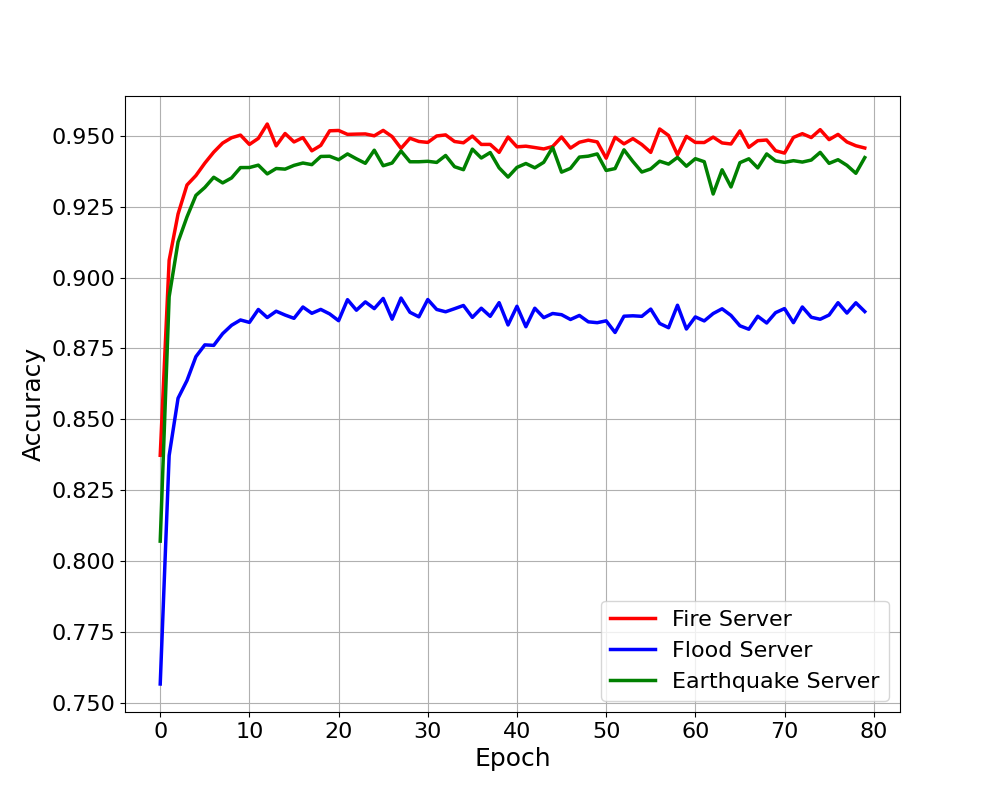
\includegraphics[width=0.75\textwidth]{figures/chapter2/User_Accuracies.png}
    \caption{Ακρίβεια κόμβων ανά εποχή}
    \label{fig1}
\end{figure}

\begin{figure}[H]
    \centering
    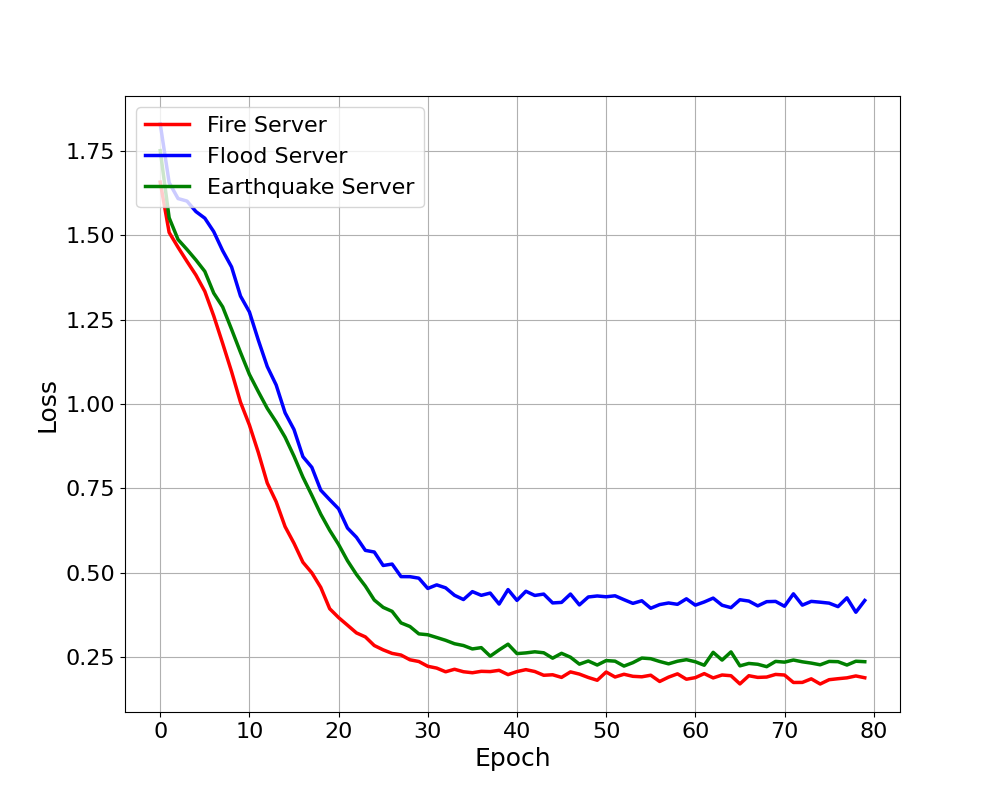
\includegraphics[width=0.75\textwidth]{figures/chapter2/User_Losses.png}
    \caption{Απώλεια κόμβων ανά εποχή}
    \label{fig2}
\end{figure}

\newpage

Όπως φαίνεται στα διαγράμματα \ref{fig1} και \ref{fig2} οι κόμβοι μας ξεκινούν την εκμάθηση και σταδιακά αφομοιώνουν την πληροφορία του παγκόσμιου μοντέλου, μαθαίνοντας και από τους υπόλοιπους κόμβους. Έτσι, η μέση ακρίβεια των κόμβων αυξάνεται σταδιακά, ενόσω κάθε κόμβος επεξεργάζεται ξανά τα δικά του δεδομένα σε συνδυασμό με την πληροφορία που δέχεται από τον εξυπηρετητή του, ενώ η απώλεια αντίστοιχα μειώνεται. Βλέπουμε πως μετά από περίπου 20 εποχές - επαναλήψεις αρχίζουν και οι δύο ποσότητες να σταθεροποιούνται καταλήγοντας σε σύγκλιση.

Αντίστοιχη συμπεριφορά παρατηρούμε στα διαγράμματα για τους Εξυπηρετητές. Η εξέταση της απόδοσης των εξυπηρετητών κατά τις εποχές παρουσιάζει μια συνεπή τάση, με τον Εξυπηρετητή Πυρκαγιάς να επιτυγχάνει σταθερά τη μεγαλύτερη ακρίβεια, ακολουθούμενος από τους Εξυπηρετητές Σεισμών και Πλημμυρών (\ref{fig3}), δεδομένου ότι ο Εξυπηρετητής Πυρκαγιάς διαθέτει μεγαλύτερο σύνολο δεδομένων και, κατά συνέπεια, επιδεικνύει ανώτερη απόδοση. Ωστόσο, μια ενδιαφέρουσα απόκλιση παρατηρείται στον Εξυπηρετητή Πλημμυρών, ο οποίος, παρά το γεγονός ότι διαθέτει μεγαλύτερο σύνολο δεδομένων σε σύγκριση με τον Εξυπηρετητή Σεισμών, παρουσιάζει χαμηλότερη απόδοση (\ref{fig3} – \ref{fig4}). Αυτή η ανωμαλία προκύπτει από τη συμπερίληψη εικόνων με περιεχόμενο νερού στα ουδέτερα σύνολα δεδομένων που μοιράζονται οι Εξυπηρετητές. Αυτές οι εικόνες εισάγουν σύγχυση στη διαδικασία εκπαίδευσης του Εξυπηρετητή Πλημμυρών, επηρεάζοντας τελικά αρνητικά την απόδοσή του. Όπως αναφέρουν και οι Barry et al. (\lcite{barry2023impact}) η ποιότητα των δεδομένων και ο θόρυβος μπορούν να επηρεάσουν σημαντικά την απόδοση του μοντέλου. Ειδικότερα αν οι καλοί κόμβοι του Εξυπηρετητή Πλημμυρών διαθέτουν παρεμφερείς εικόνες με αυτές του Ουδέτερου Συνόλου Δεδομένων η εκμάθηση γίνεται πολύ δύσκολη αφού αυτοί οι κόμβοι έχουν τη μεγαλύτερη συμμετοχή στη διαδικασία.

\begin{figure}[ht]
    \centering
    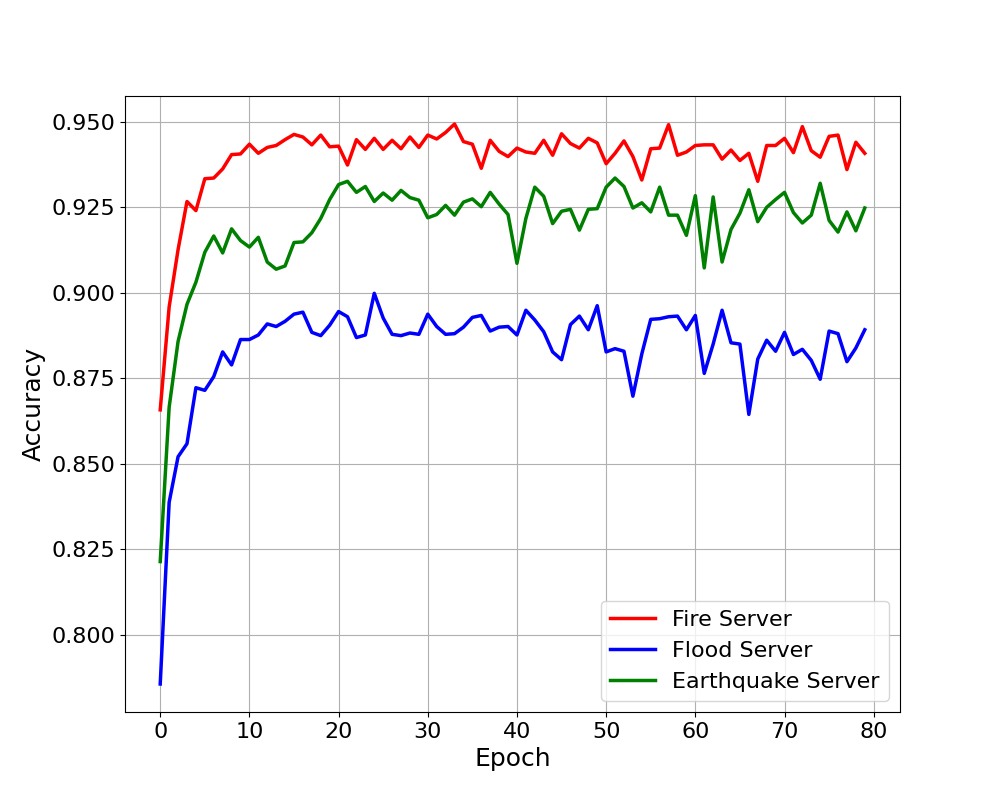
\includegraphics[width=0.75\textwidth]{figures/chapter2/Server_Accuracies.png}
    \caption{Ακρίβεια Εξυπηρετητών ανά εποχή}
    \label{fig3}
\end{figure}

\newpage

\begin{figure}[ht]
    \centering
    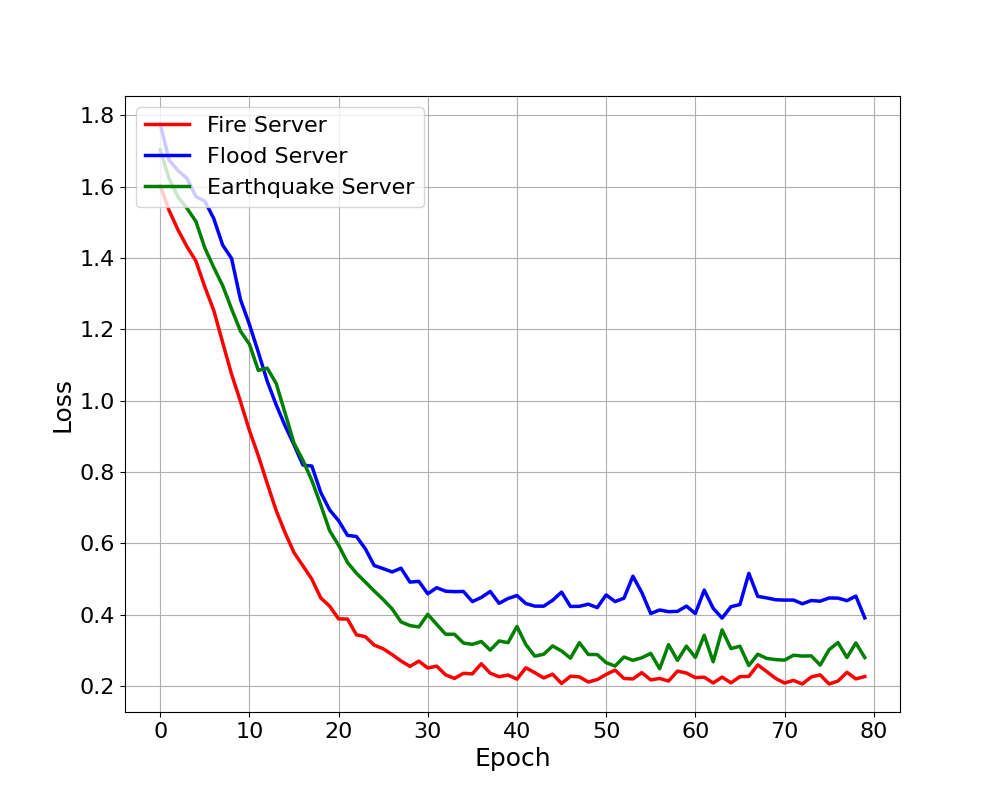
\includegraphics[width=0.75\textwidth]{figures/chapter2/Server_Losses.png}
    \caption{Απώλεια Εξυπηρετητών ανά εποχή}
    \label{fig4}
\end{figure}

Έτσι, ο Εξυπηρετητής Σεισμών, παρά το μικρότερο σύνολο δεδομένων, αποδίδει σχετικά καλύτερα από το αναμενόμενο, καταδεικνύοντας την πολύπλοκη σχέση μεταξύ μεγέθους συνόλου δεδομένων και απόδοσης. Επίσης, οι κόμβοι που σχετίζονται με τον Εξυπηρετητή Σεισμών επιτυγχάνουν σταθερά υψηλότερη τοπική ακρίβεια σε σύγκριση με τους κόμβους των Εξυπηρετητών Πυρκαγιάς και Πλημμυρών (\ref{fig1}), αποδεικνύοντας την αποτελεσματικότητα των αντίστοιχων συνόλων δεδομένων. Ωστόσο, η διαφορά στην απόδοση των κόμβων δεν αντικατοπτρίζει άμεσα την ιεραρχία που παρατηρείται στην απόδοση των Εξυπηρετητών. Αυτή η απόκλιση προκύπτει από τη δυσκολία της πραγματικής σύνθεσης των συνόλων των παραμέτρων στο παγκόσμιο μοντέλο, αλλά και από υπερπροσαρμογή των κόμβων του Εξυπηρετητή Σεισμών (διαφορά μεταξύ ακρίβειας εκπαίδευσης και ακρίβειας δοκιμών).

\newpage

\begin{figure}[H]
    \centering
    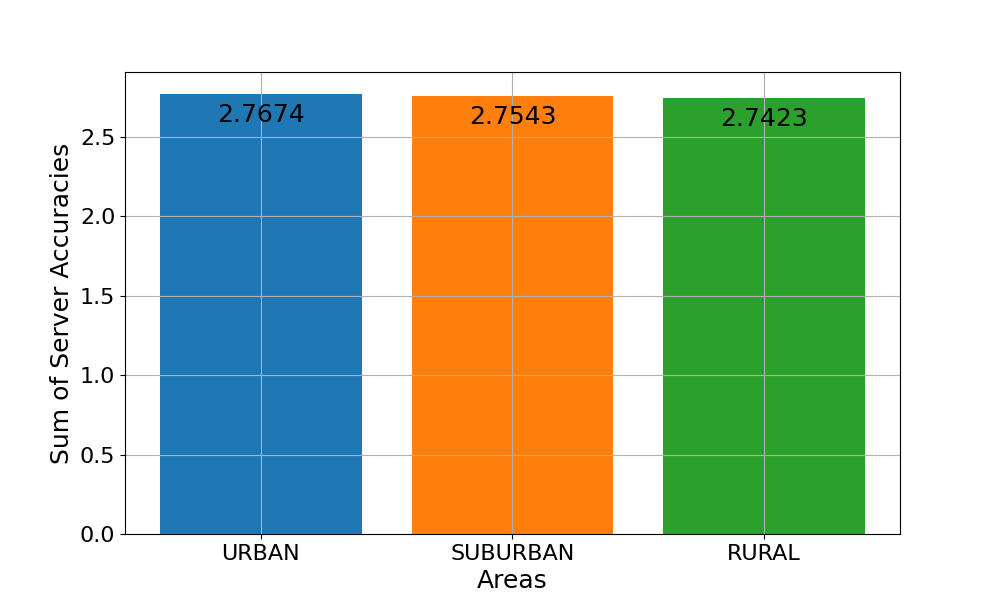
\includegraphics[width=\textwidth]{figures/chapter2/Sum_of_Accuracies_per_Area.png}
    \caption{Σενάριο Δημόσιας ασφάλειας σε διαφορετικές περιοχές (αστική, προαστική, αγροτική) - Ακρίβεια}
    \label{fig5}
\end{figure}

\begin{figure}[H]
    \centering
    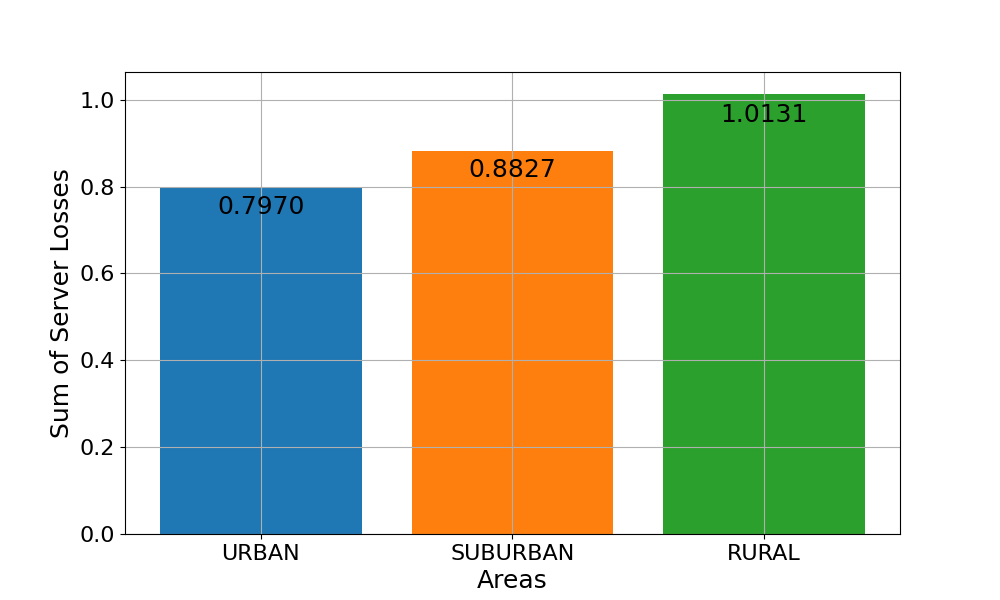
\includegraphics[width=\textwidth]{figures/chapter2/Sum_of_Losses_per_Area.png}
    \caption{Σενάριο Δημόσιας ασφάλειας σε διαφορετικές περιοχές (αστική, προαστική, αγροτική) - Απώλεια}
    \label{fig6}
\end{figure}

\newpage

Ο μηχανισμός αντιστοίχισης δοκιμάζεται σε ένα ρεαλιστικό σενάριο δημόσιας ασφάλειας σε αστικά, προαστιακά και αγροτικά περιβάλλοντα. Η \ref{fig5} παρουσιάζει το άθροισμα της ακρίβειας των εξυπηρετητών για τρία διακριτά σενάρια: Αστικό, Προαστιακό και Αγροτικό, καθένα από τα οποία χαρακτηρίζεται από διαφορετική σύνθεση κόμβων. Αντίστοιχα στο \ref{fig6} παρουσιάζει το άθροισμα της απώλειας των εξυπηρετητών στις τρεις αυτές περιοχές.

Σε κάθε σενάριο, οι κόμβοι κατηγοριοποιούνται είτε ως καλοί (κοντά στα Σημεία Ενδιαφέροντος) είτε ως κακοί (μακριά από τα Σημεία Ενδιαφέροντος, γεγονός που οδηγεί σε σύγχυση του αλγορίθμου και μειωμένη χρησιμότητα δεδομένων). Το όριο που διαχωρίζει τους καλούς από τους κακούς κόμβους διαφέρει μεταξύ των σεναρίων: Αστικό (30), Προαστιακό (21) και Αγροτικό (12), υποδεικνύοντας το σημείο πέρα από το οποίο οι κόμβοι θεωρούνται κακοί.

Τα αποτελέσματα αποκαλύπτουν ένα συνεπές πρότυπο για τα τρία σενάρια. Όσο οι κόμβοι μας είναι πιο απομακρυσμένοι από τα σημεία ενδιαφέροντος και άρα διαθέτουν λιγότερη πληροφορία, καθιστούν πιο δύσκολη την εκπαίδευση του κεντρικού μοντέλου. Για αυτό το λόγο, όπως φαίνεται, πετυχαίνουμε καλύτερη αθροιστική Ακρίβεια και μικρότερη σε μία Αστική Περιοχή απ' ότι σε μία Προαστιακή Περιοχή και μία Αγροτική Περιοχή. 

Από τη συμπεριφορά αυτή φαίνεται πώς η διαφοροποίηση ανά περιοχή με καλούς και κακούς κόμβους επηρεάζει την εκμάθηση των μοντέλων. Έχοντας κόμβους με λιγότερα δεδομένα - εικόνες να συμμετέχουν στην Ομοσπονδιακή Μάθηση, δυσκολεύει σε κάποιο βαθμό τη γενίκευση στο παγκόσμιο μοντέλο. Η αρνητική επίδραση αυτή καταπολεμάται από τον αλγόριθμό μας με τη χρήση βαρών συμμετοχής στην εκμάθηση, όπου ένας κακός κόμβος, με λιγότερα, άρα και πιο μη γενικευμένα δεδομένα, συμμετέχει λιγότερο σε σχέση με έναν κόμβο που διαθέτει περισσότερη πληροφορία, με αποτέλεσμα εν τέλει σε όλες τις περιοχές να πετυχαίνουμε πολύ καλά αποτελέσματα για τα παγκόσμια μοντέλα.
